
The performances on the test videos are summarized in Table~\ref{Results:tab:video1} and Table~\ref{Results:tab:video2}, while some qualitative results are shown in Figure~\ref{Results:fig:video1} and Figure~\ref{Results:fig:video2}.

Analysing the results on both videos it seems that the performances are generally lower than the one obtained on images, with an average accuracy of $68.00\,\%$ on video 1 and $70.83\,\%$ on video 2.
But it can be immediately noticed from Figure~\ref{Results:fig:video1_frame0} and Figure~\ref{Results:fig:video2_frame2} that the hand was covering almost all the coins, making the detection task impossible.
Excluding these frames from the evaluation, the average accuracy rises to $82.50\,\%$ on video 1 and $88.54\,\%$ on video 2 which is more in line with the results obtained on images.

As said for the test images, our method is not immune to strong light reflections.
This is particularly emphasized in videos because of the flickering effect, which consists of rapid changes in brightness and non-uniform lighting.
Flickering occurs because the light source is synchronized with the alternating current, while the camera is unable to capture a perfectly stable image.

Another observation from the video results is that overlapping coins are particularly difficult to detect.
This is not because they are not recognized as circles, but rather because the template matching step often fails to identify them correctly, likely due to mutual shadowing and partial occlusion of coin details.

\begin{table}[H]
\centering
\begin{tabular}{c|c|c|c|c}
\toprule
\textbf{Frames} & \textbf{mIoU} & \textbf{Accuracy} & \textbf{Predicted sum} & \textbf{Sum error} \\[4pt]
\midrule
frame a     & $0.110$     & $10.00\,\%$     & $2.00$     & $-7.22$ \\[8pt]
frame b     & $0.851$     & $90.90\,\%$     & $9.70$     & $-0.02$ \\[8pt]
frame c     & $0.884$     & $84.62\,\%$     & $10.0$     & $-0.32$ \\[8pt]
frame d     & $0.827$     & $85.71\,\%$     & $9.83$     & $-0.20$ \\[8pt]
frame e     & $0.702$     & $68.75\,\%$     & $7.84$     & $-3.73$ \\
\bottomrule
\end{tabular}
\caption{Performance metrics for reference frames of video 1.}
\label{Results:tab:video1}
\end{table}

\setcounter{subfigure}{0} % per resettare il contatore delle subfigure
\begin{figure}[H]
    \addtocounter{figure}{1} % per non saltare il numero
    \centering
    \subfloat[\label{Results:fig:video1_frame0}]{
        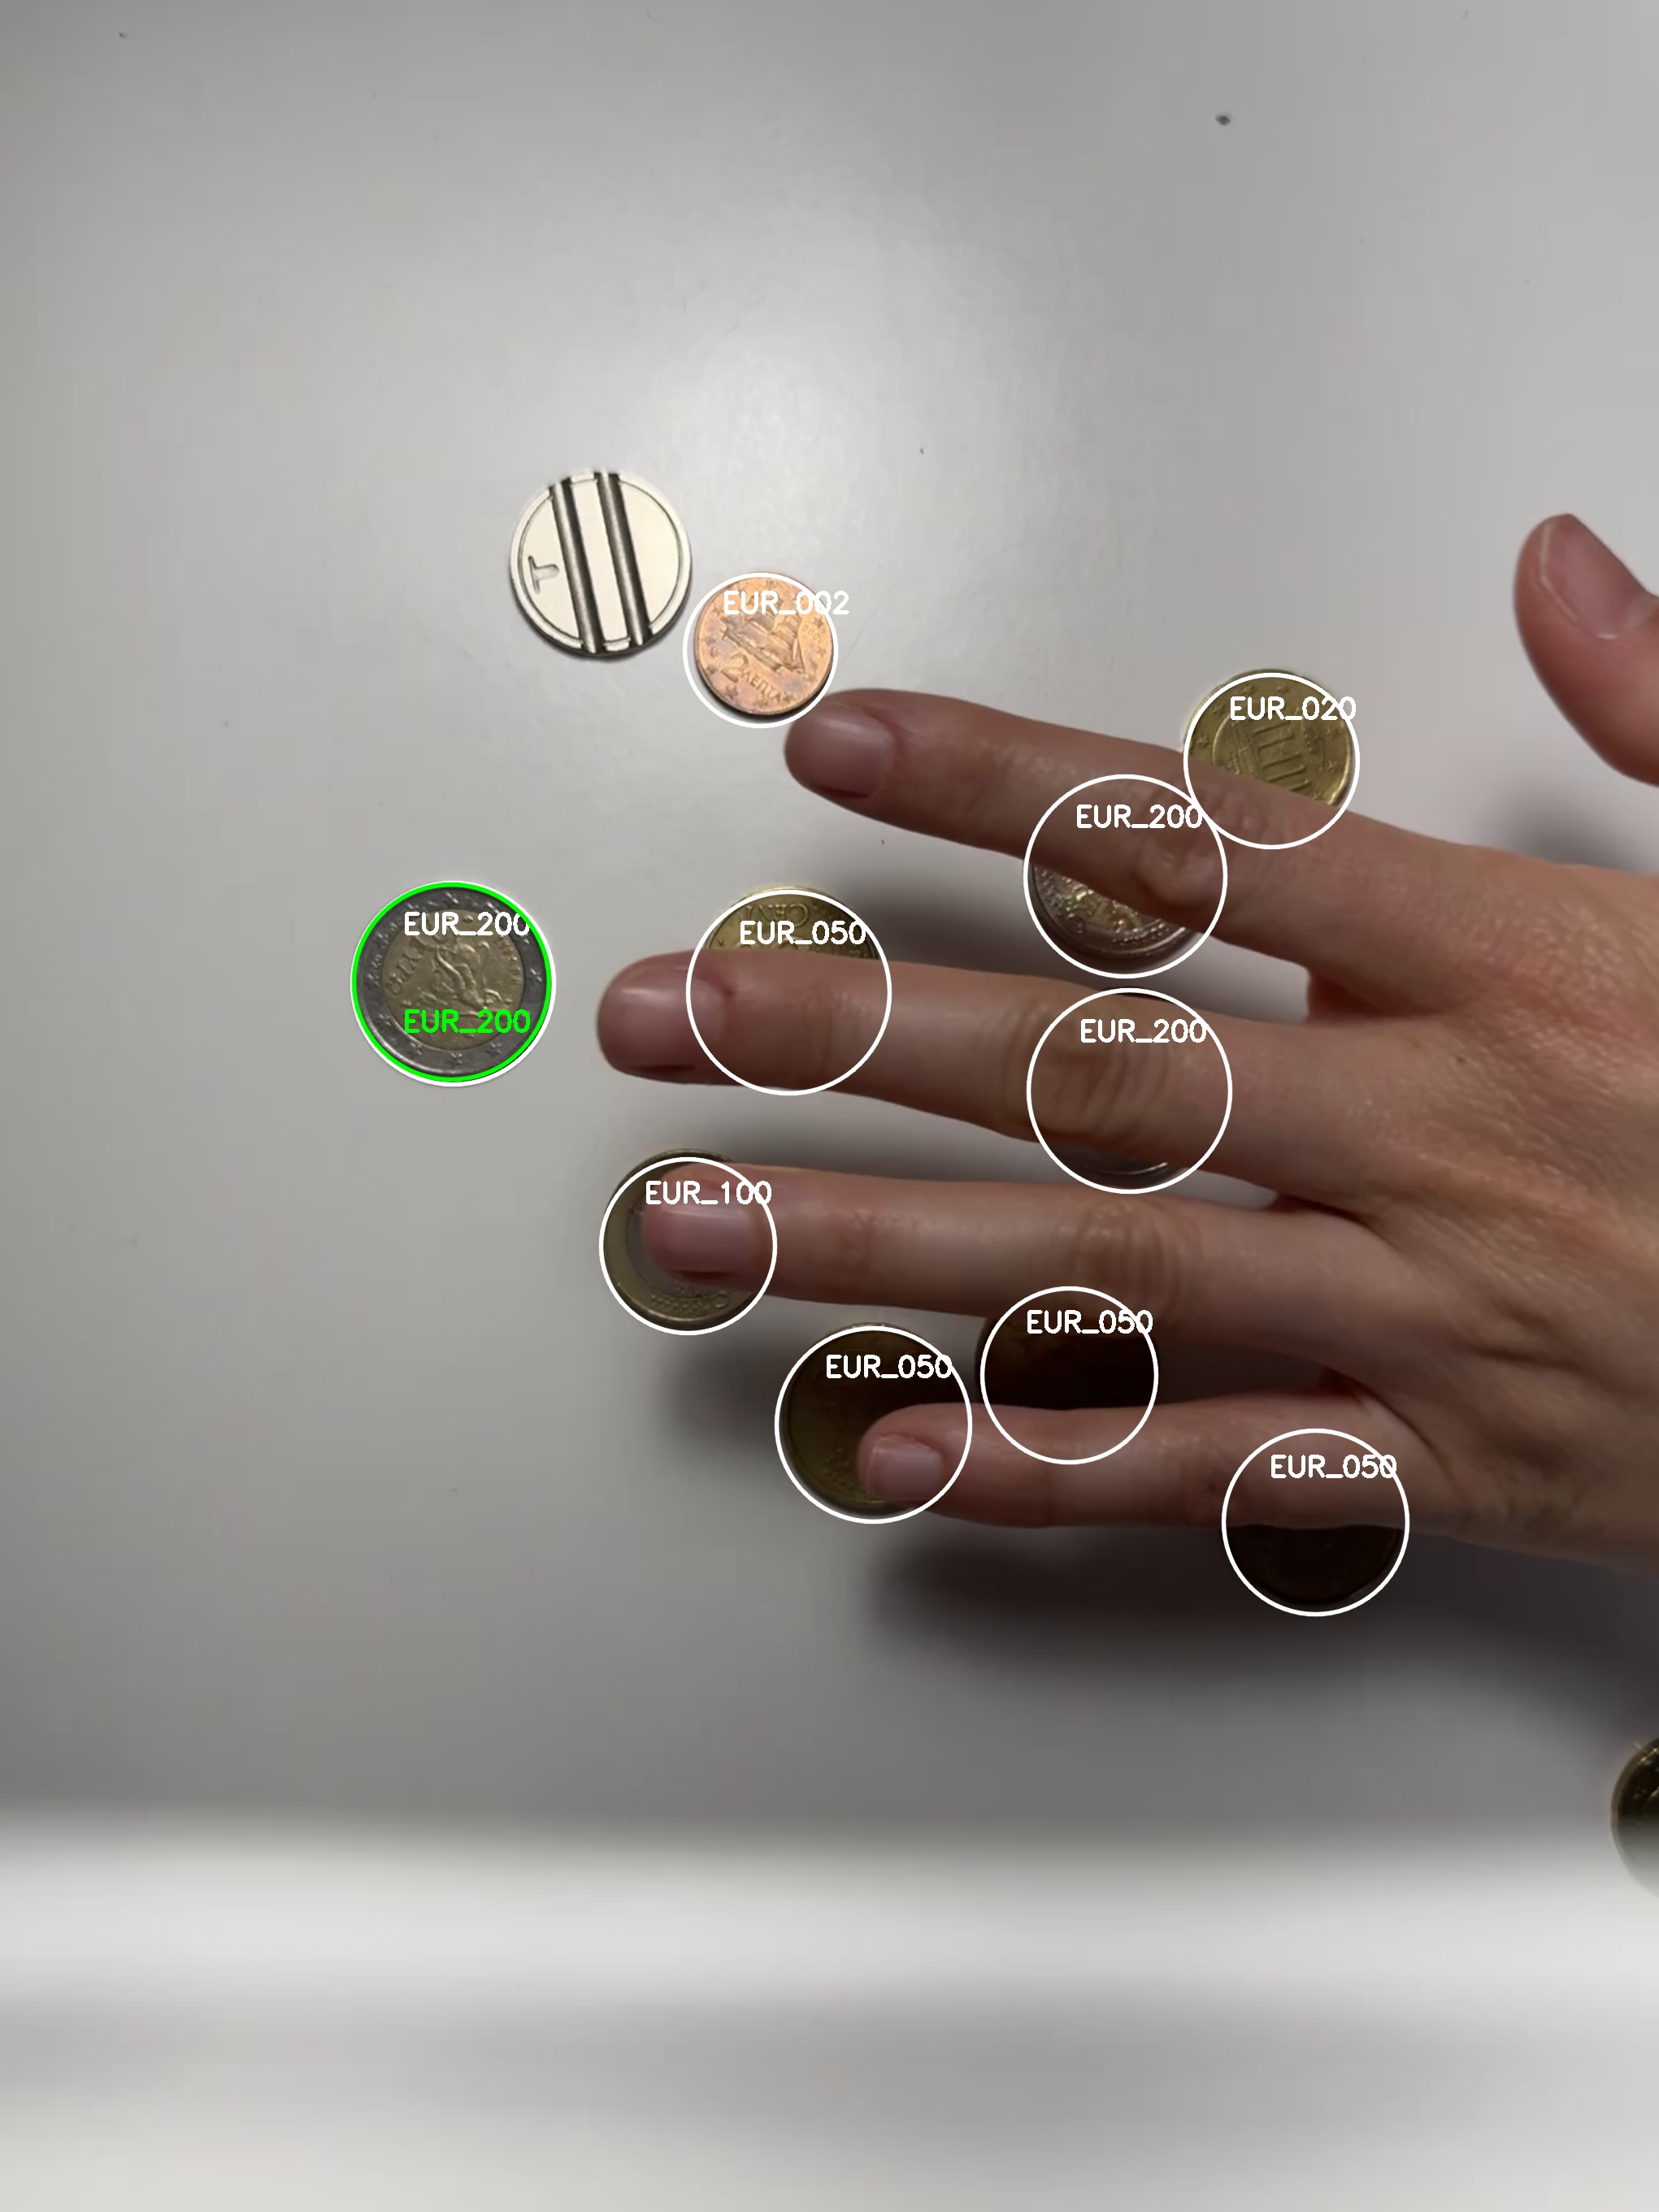
\includegraphics[width=0.45\textwidth]{Immagini/video1_frame0.jpg}
    }\hfill
    \subfloat[\label{Results:fig:video1_frame1}]{
        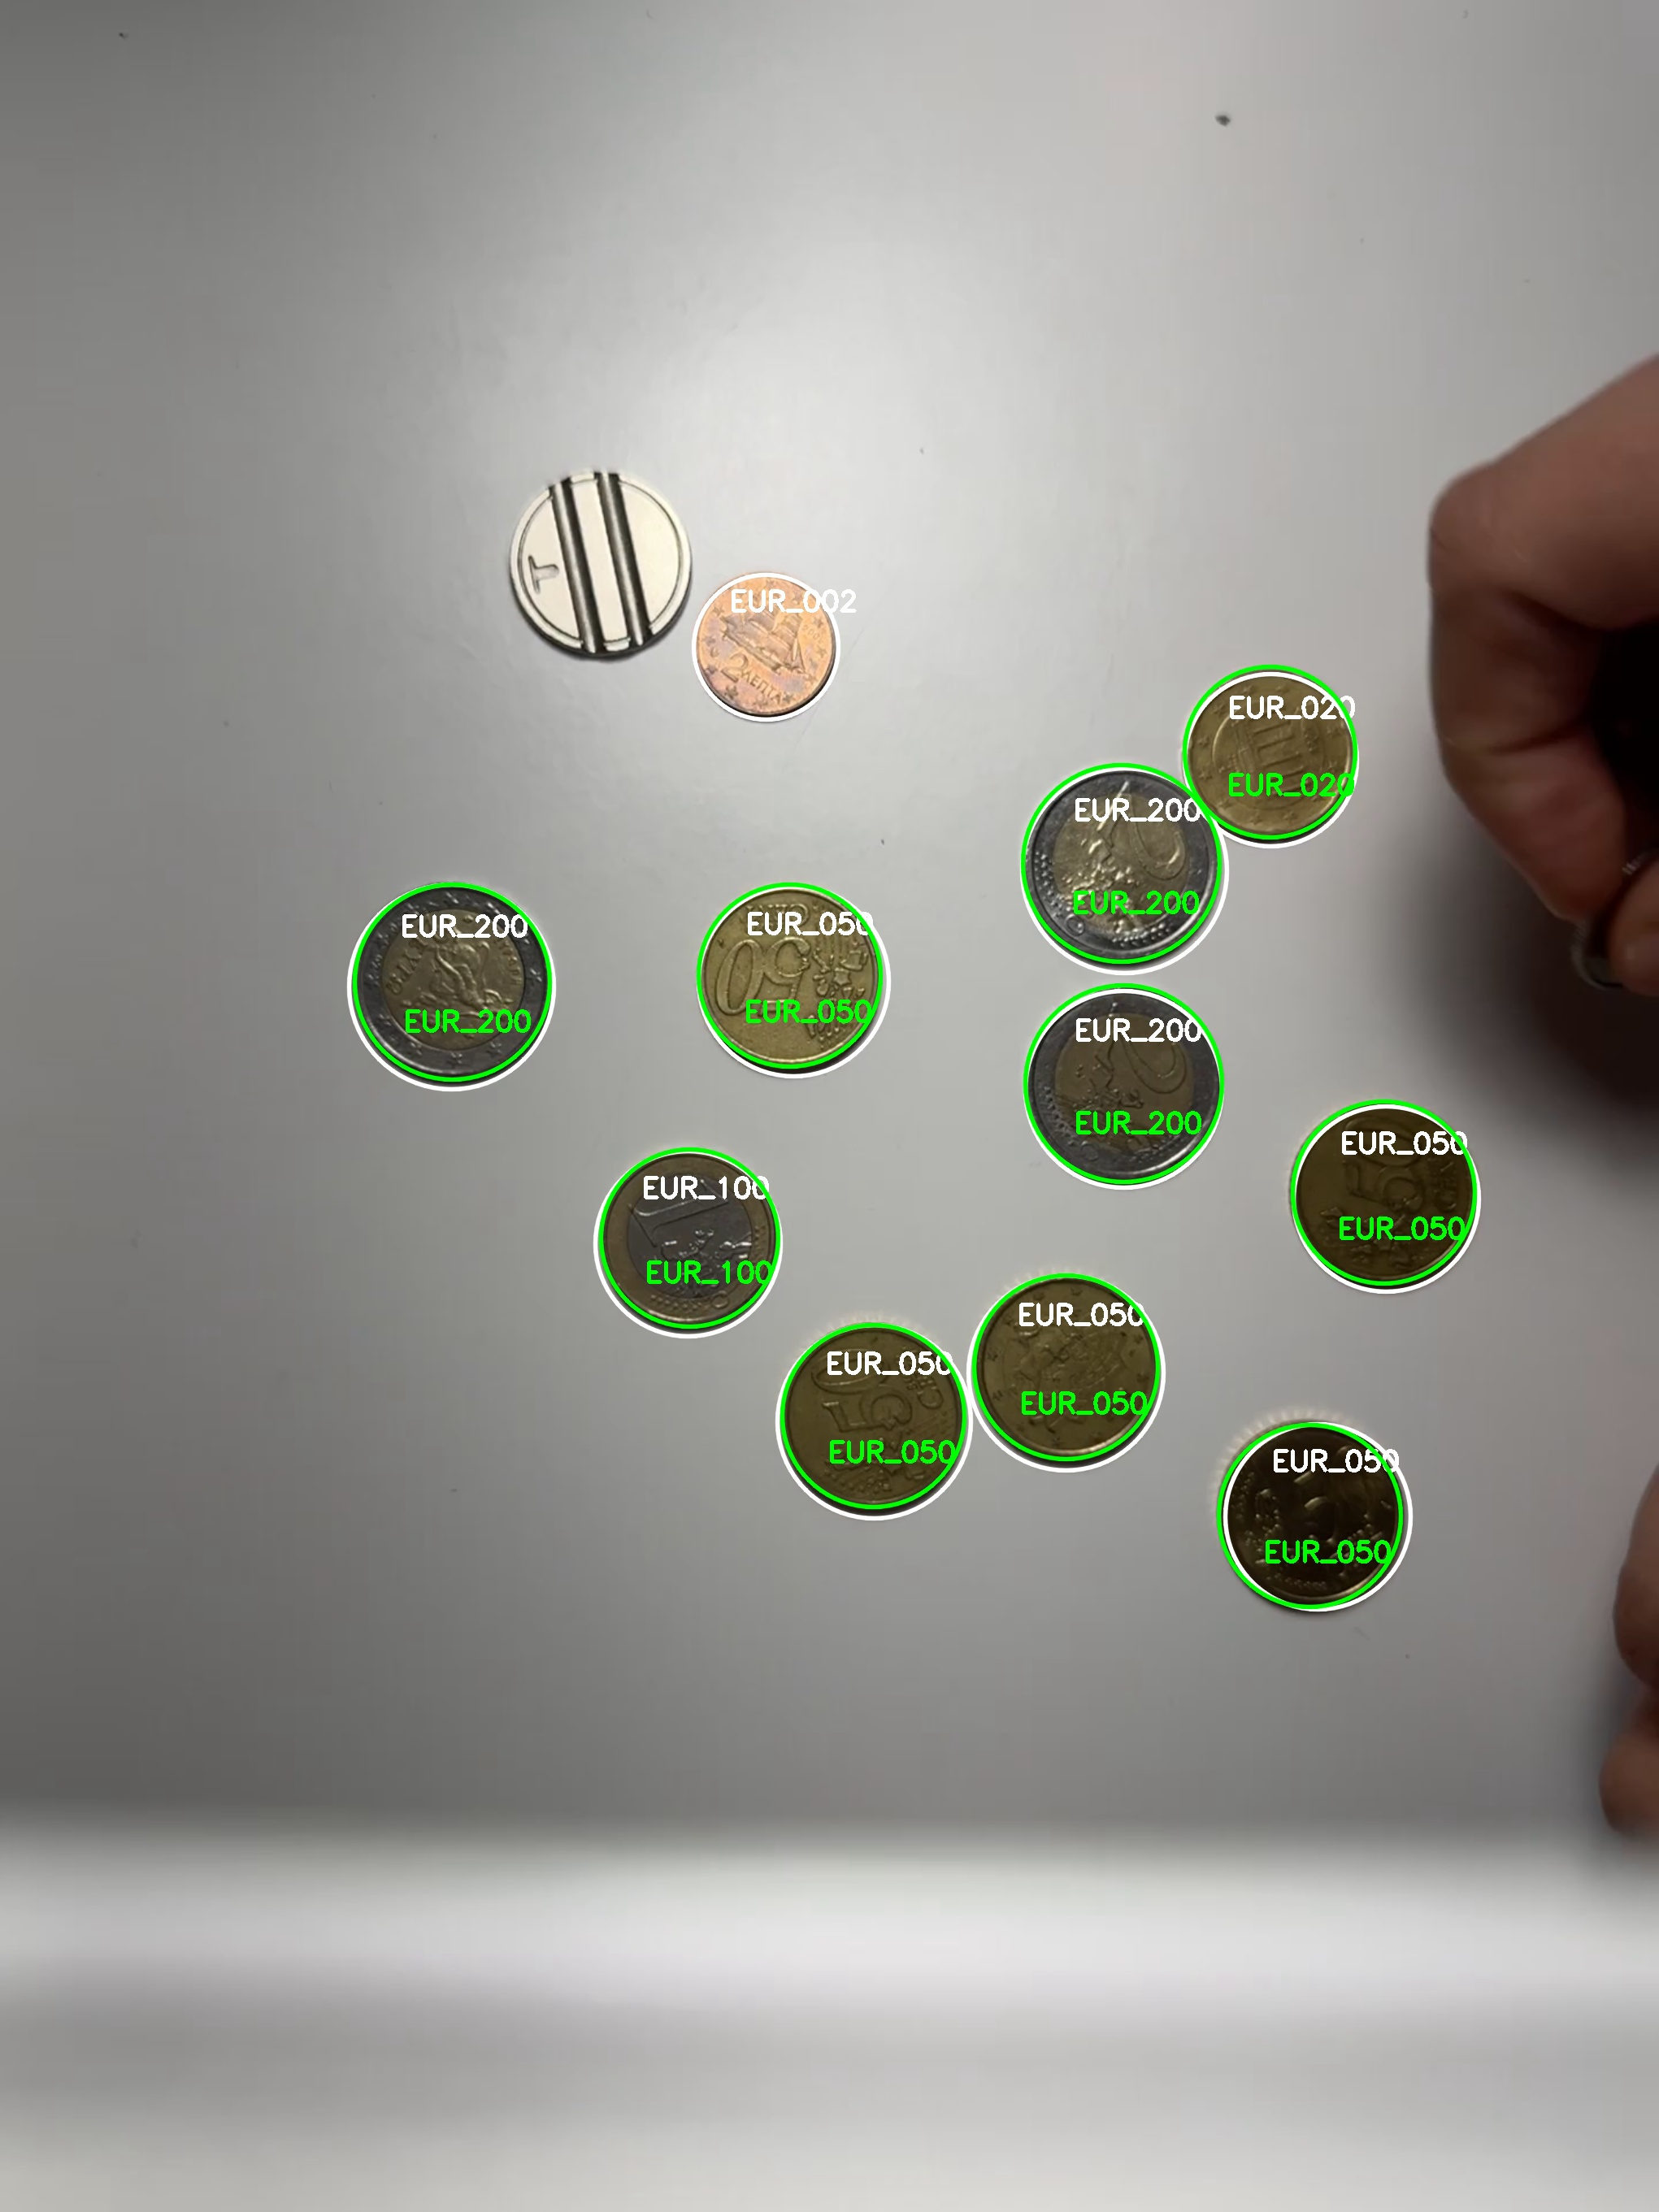
\includegraphics[width=0.45\textwidth]{Immagini/video1_frame1.jpg}
    }
\end{figure}
\begin{figure}[H]
    \addtocounter{figure}{1} % per non saltare il numero
    \ContinuedFloat
    \centering
    \subfloat[\label{Results:fig:video1_frame2}]{
        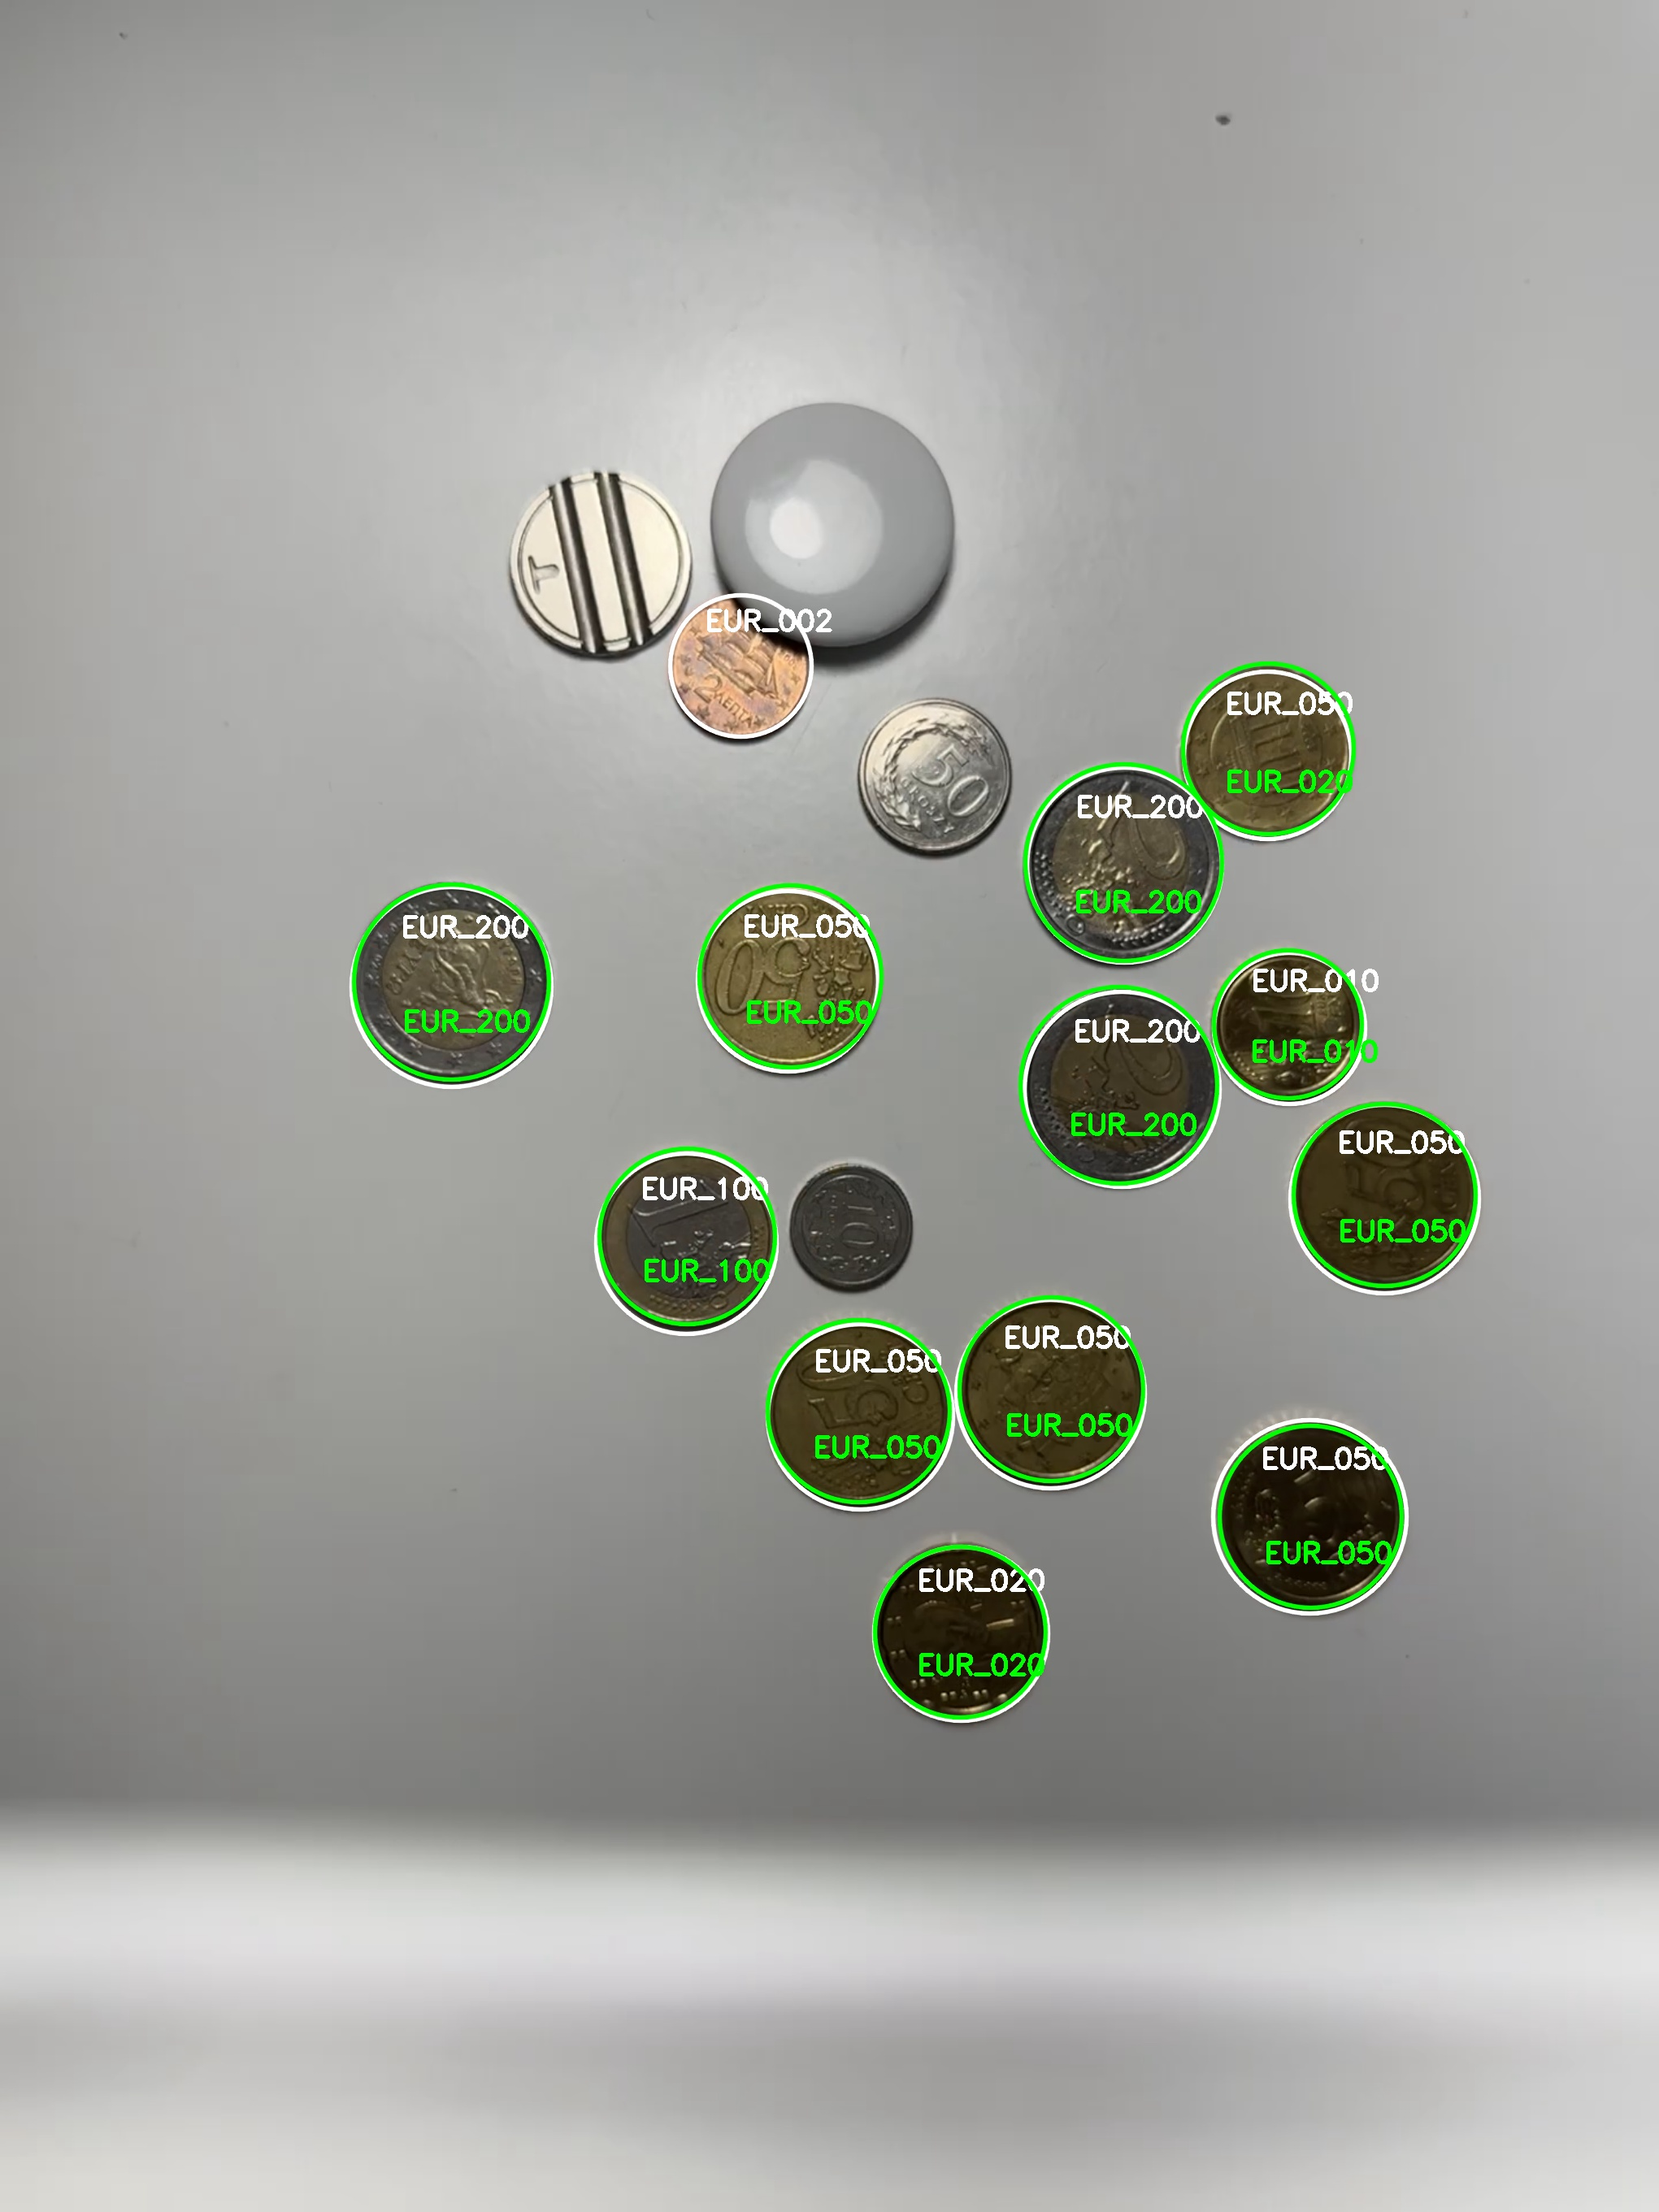
\includegraphics[width=0.45\textwidth]{Immagini/video1_frame2.jpg}
    }\hfill
    \subfloat[\label{Results:fig:video1_frame3}]{
        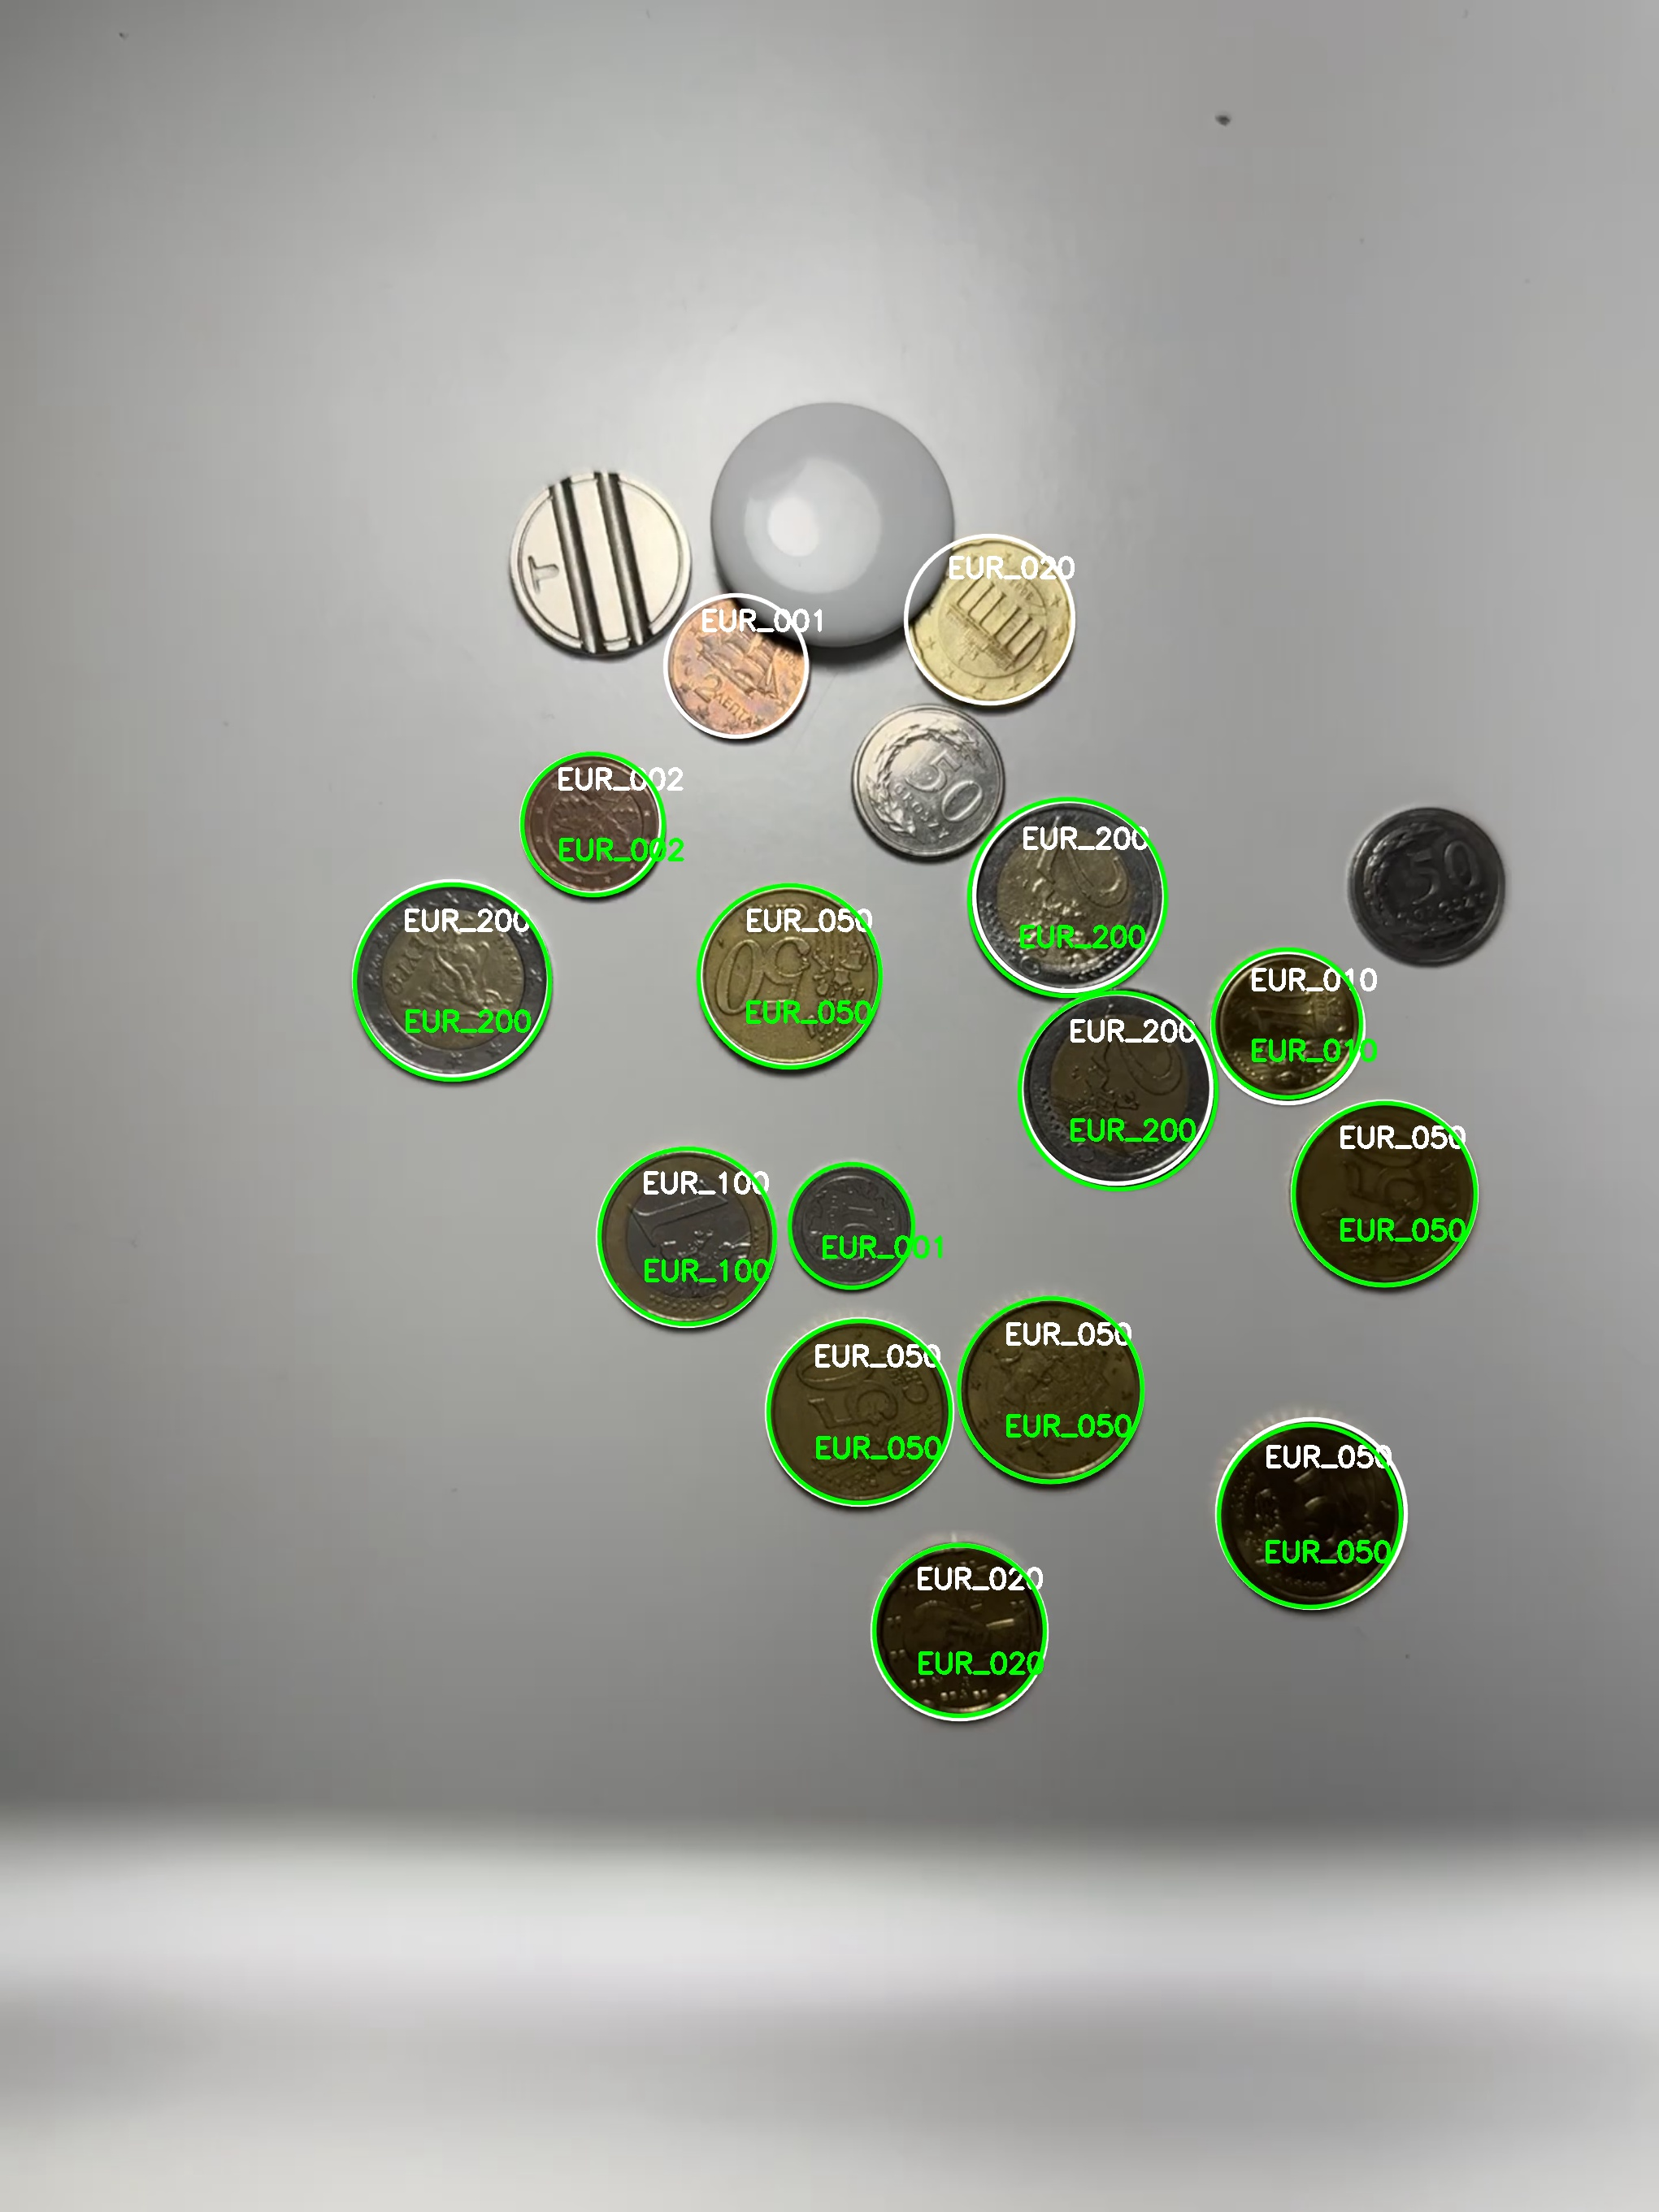
\includegraphics[width=0.45\textwidth]{Immagini/video1_frame3.jpg}
    }
\end{figure}
\begin{figure}[H]
    \ContinuedFloat
    \centering
    \subfloat[\label{Results:fig:video1_frame4}]{
        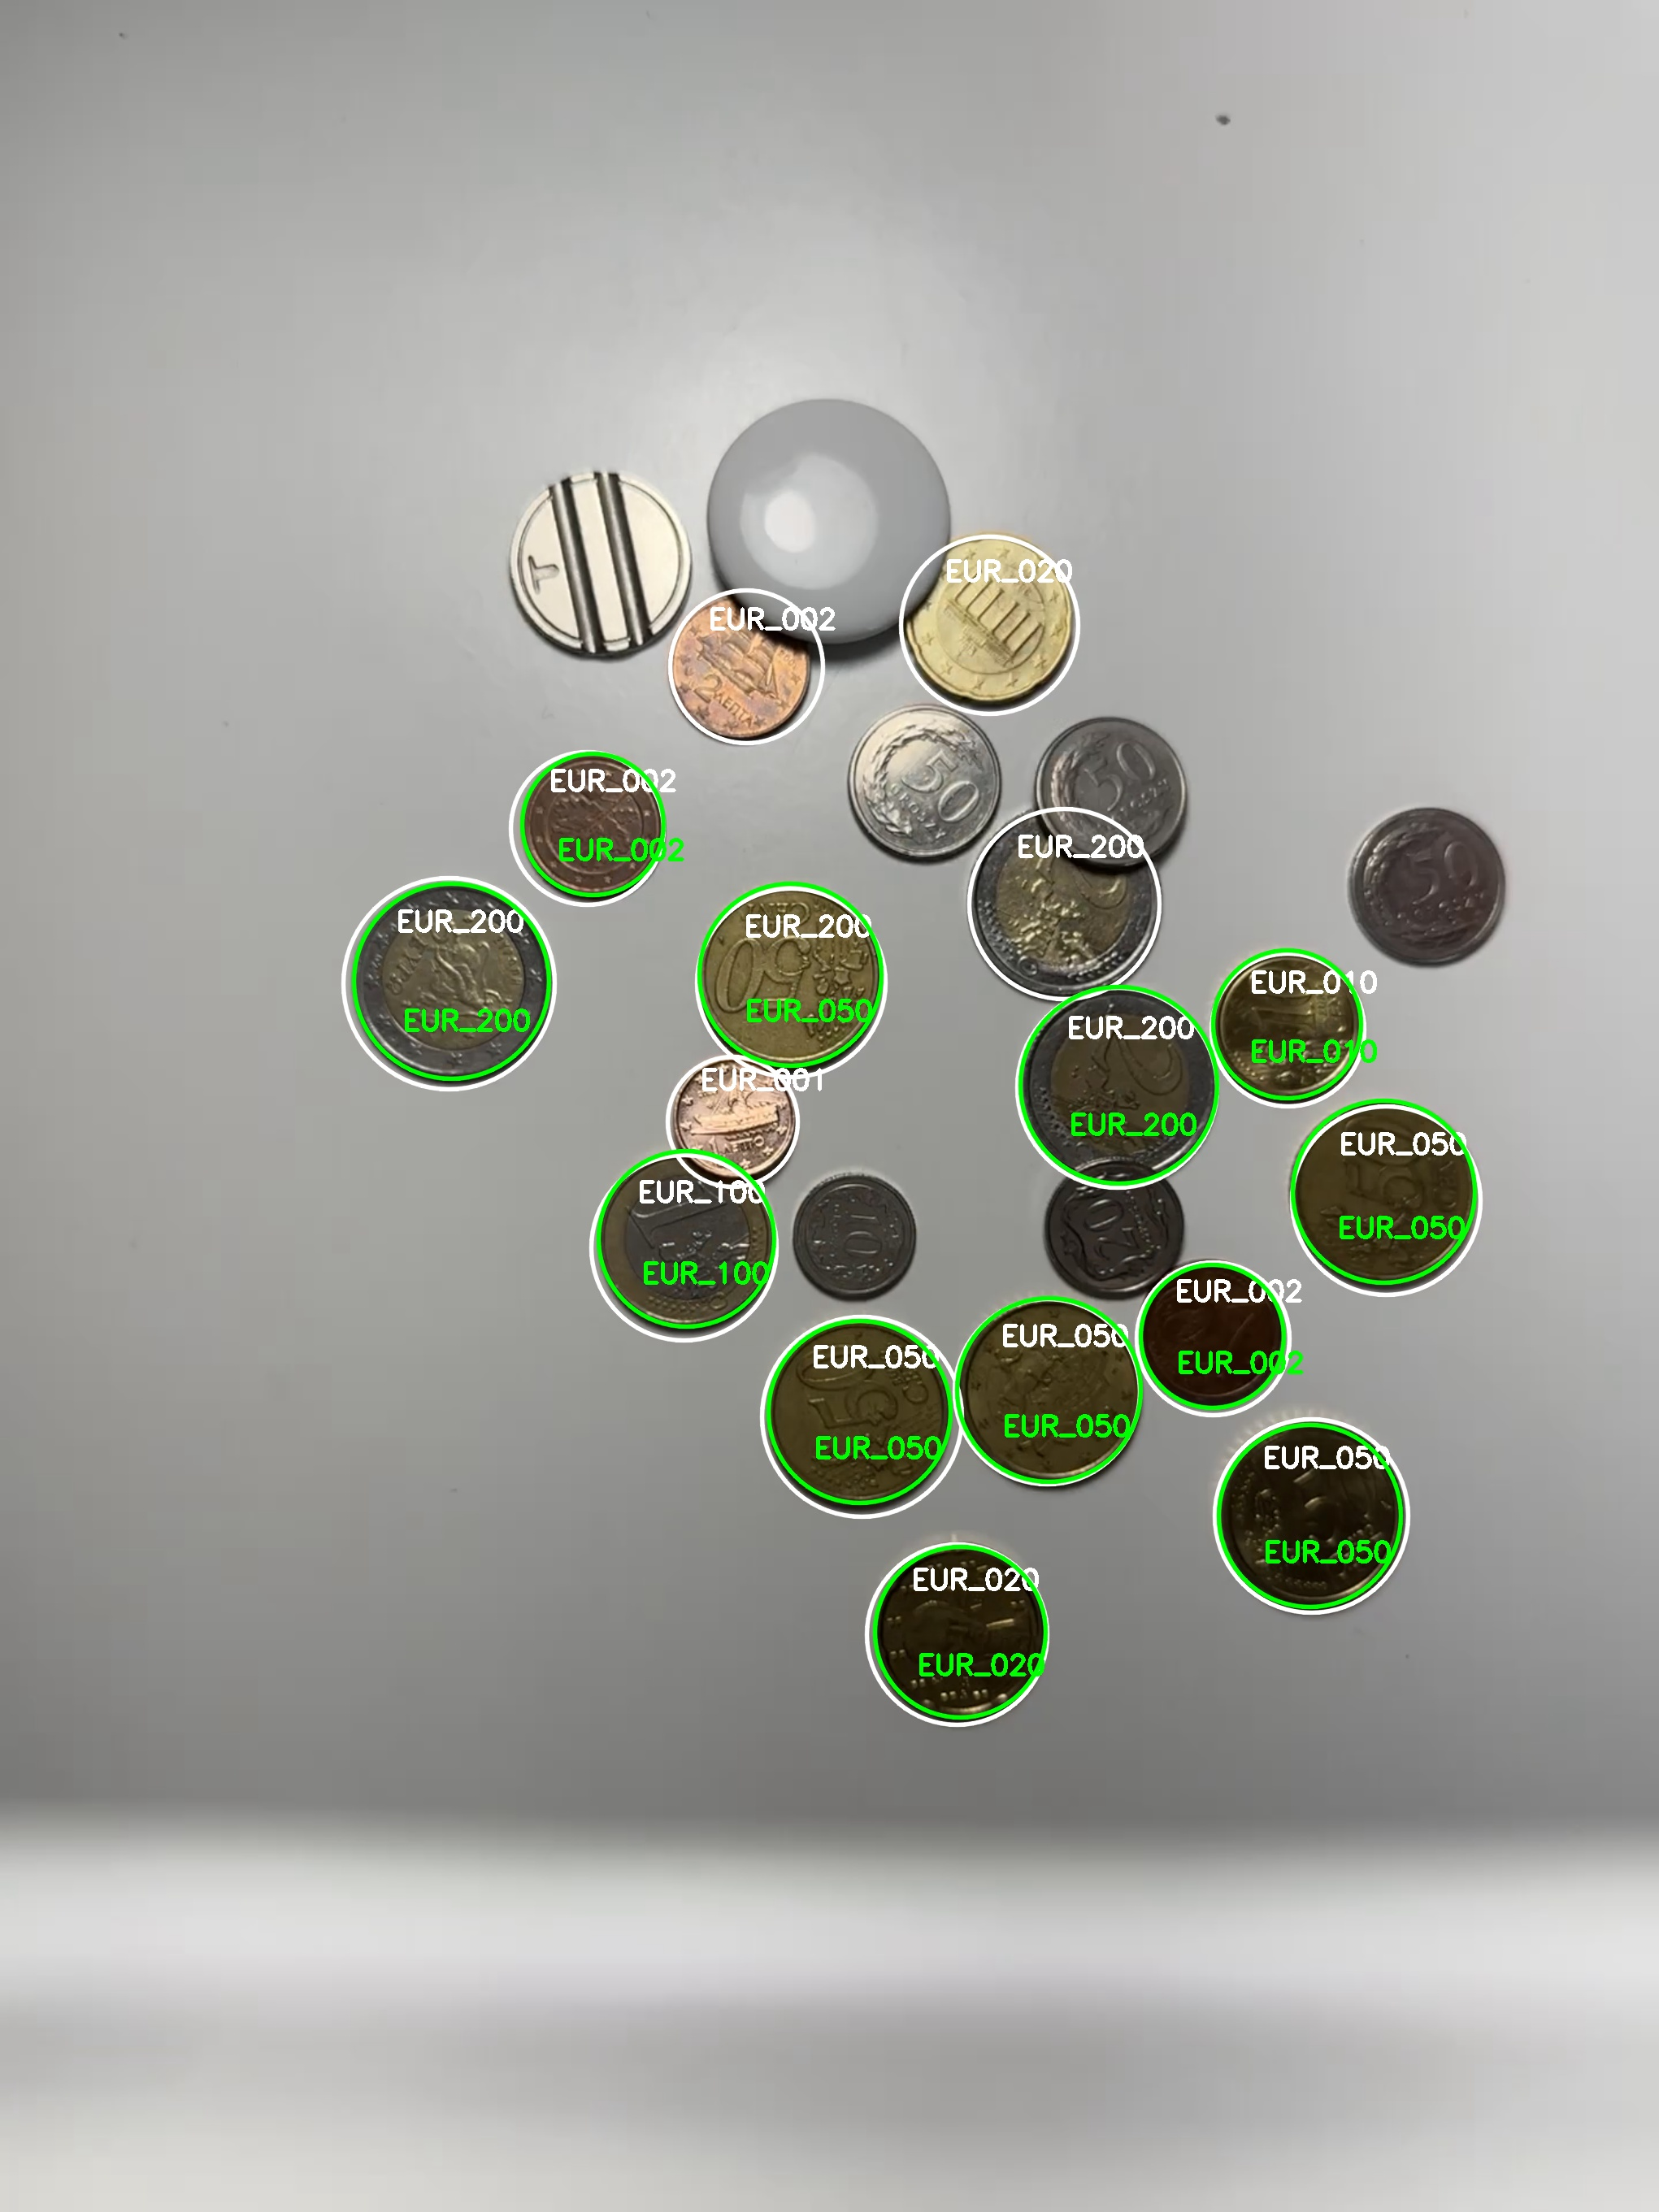
\includegraphics[width=0.45\textwidth]{Immagini/video1_frame4.jpg}
    }
    \caption{Results of the detection algorithm on selected frames from video 1.
    The ground truth circles are drawn in white, while the detected ones are drawn in green.}
    \label{Results:fig:video1}
\end{figure}

\begin{table}[H]
\centering
\begin{tabular}{c|c|c|c|c}
\toprule
\textbf{Frames} & \textbf{mIoU} & \textbf{Accuracy} & \textbf{Predicted sum} & \textbf{Sum error} \\[4pt]
\midrule
frame a     & $0.884$     & $66.67\,\%$     & $1.52$     & $+0.01$ \\[8pt]
frame b     & $0.915$     & $100.0\,\%$     & $3.51$     & $ 0.00$ \\[8pt]
frame c     & $0.000$     & $ 0.00\,\%$     & $0.00$     & $-2.53$ \\[8pt]
frame d     & $0.824$     & $100.0\,\%$     & $6.55$     & $+0.50$ \\[8pt]
frame e     & $0.845$     & $87.50\,\%$     & $8.87$     & $-1.20$ \\
\bottomrule
\end{tabular}
\caption{Performance metrics for reference frames of video 2.}
\label{Results:tab:video2}
\end{table}

\setcounter{subfigure}{0} % per resettare il contatore delle subfigure
\begin{figure}[H]
    \addtocounter{figure}{1} % per non saltare il numero
    \centering
    \subfloat[\label{Results:fig:video2_frame0}]{
        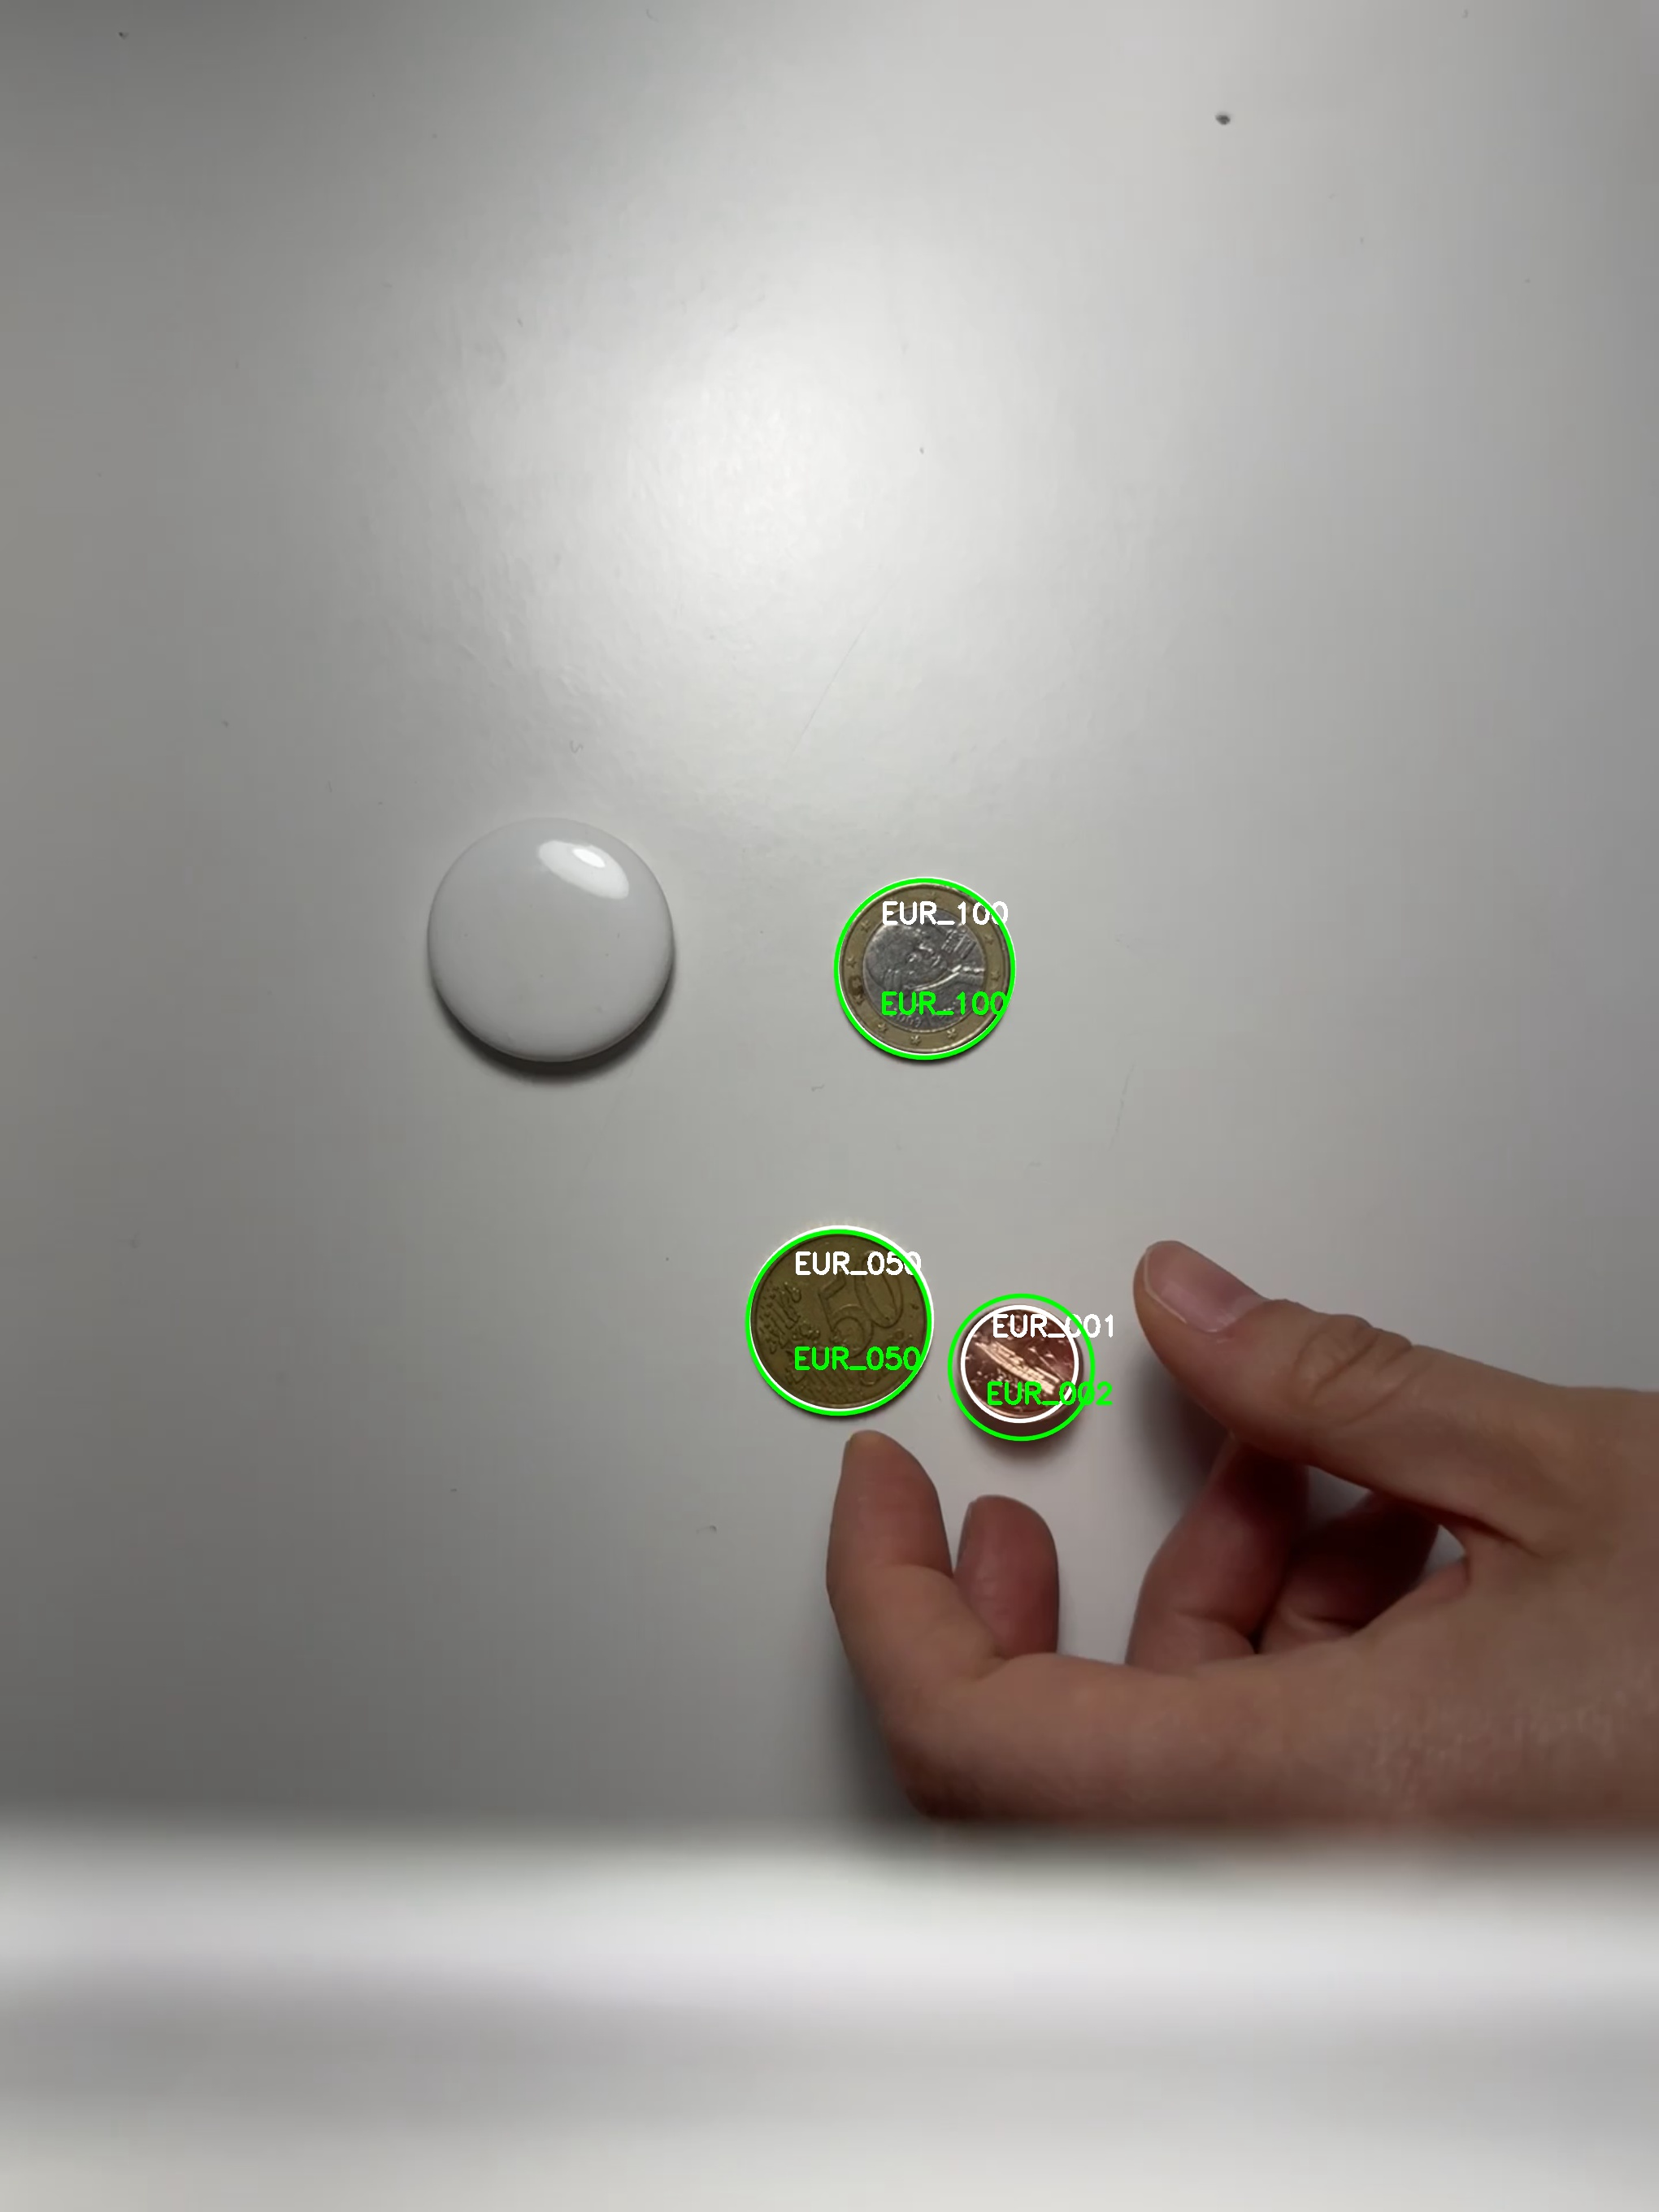
\includegraphics[width=0.45\textwidth]{Immagini/video2_frame_0.jpg}
    }\hfill
    \subfloat[\label{Results:fig:video2_frame1}]{
        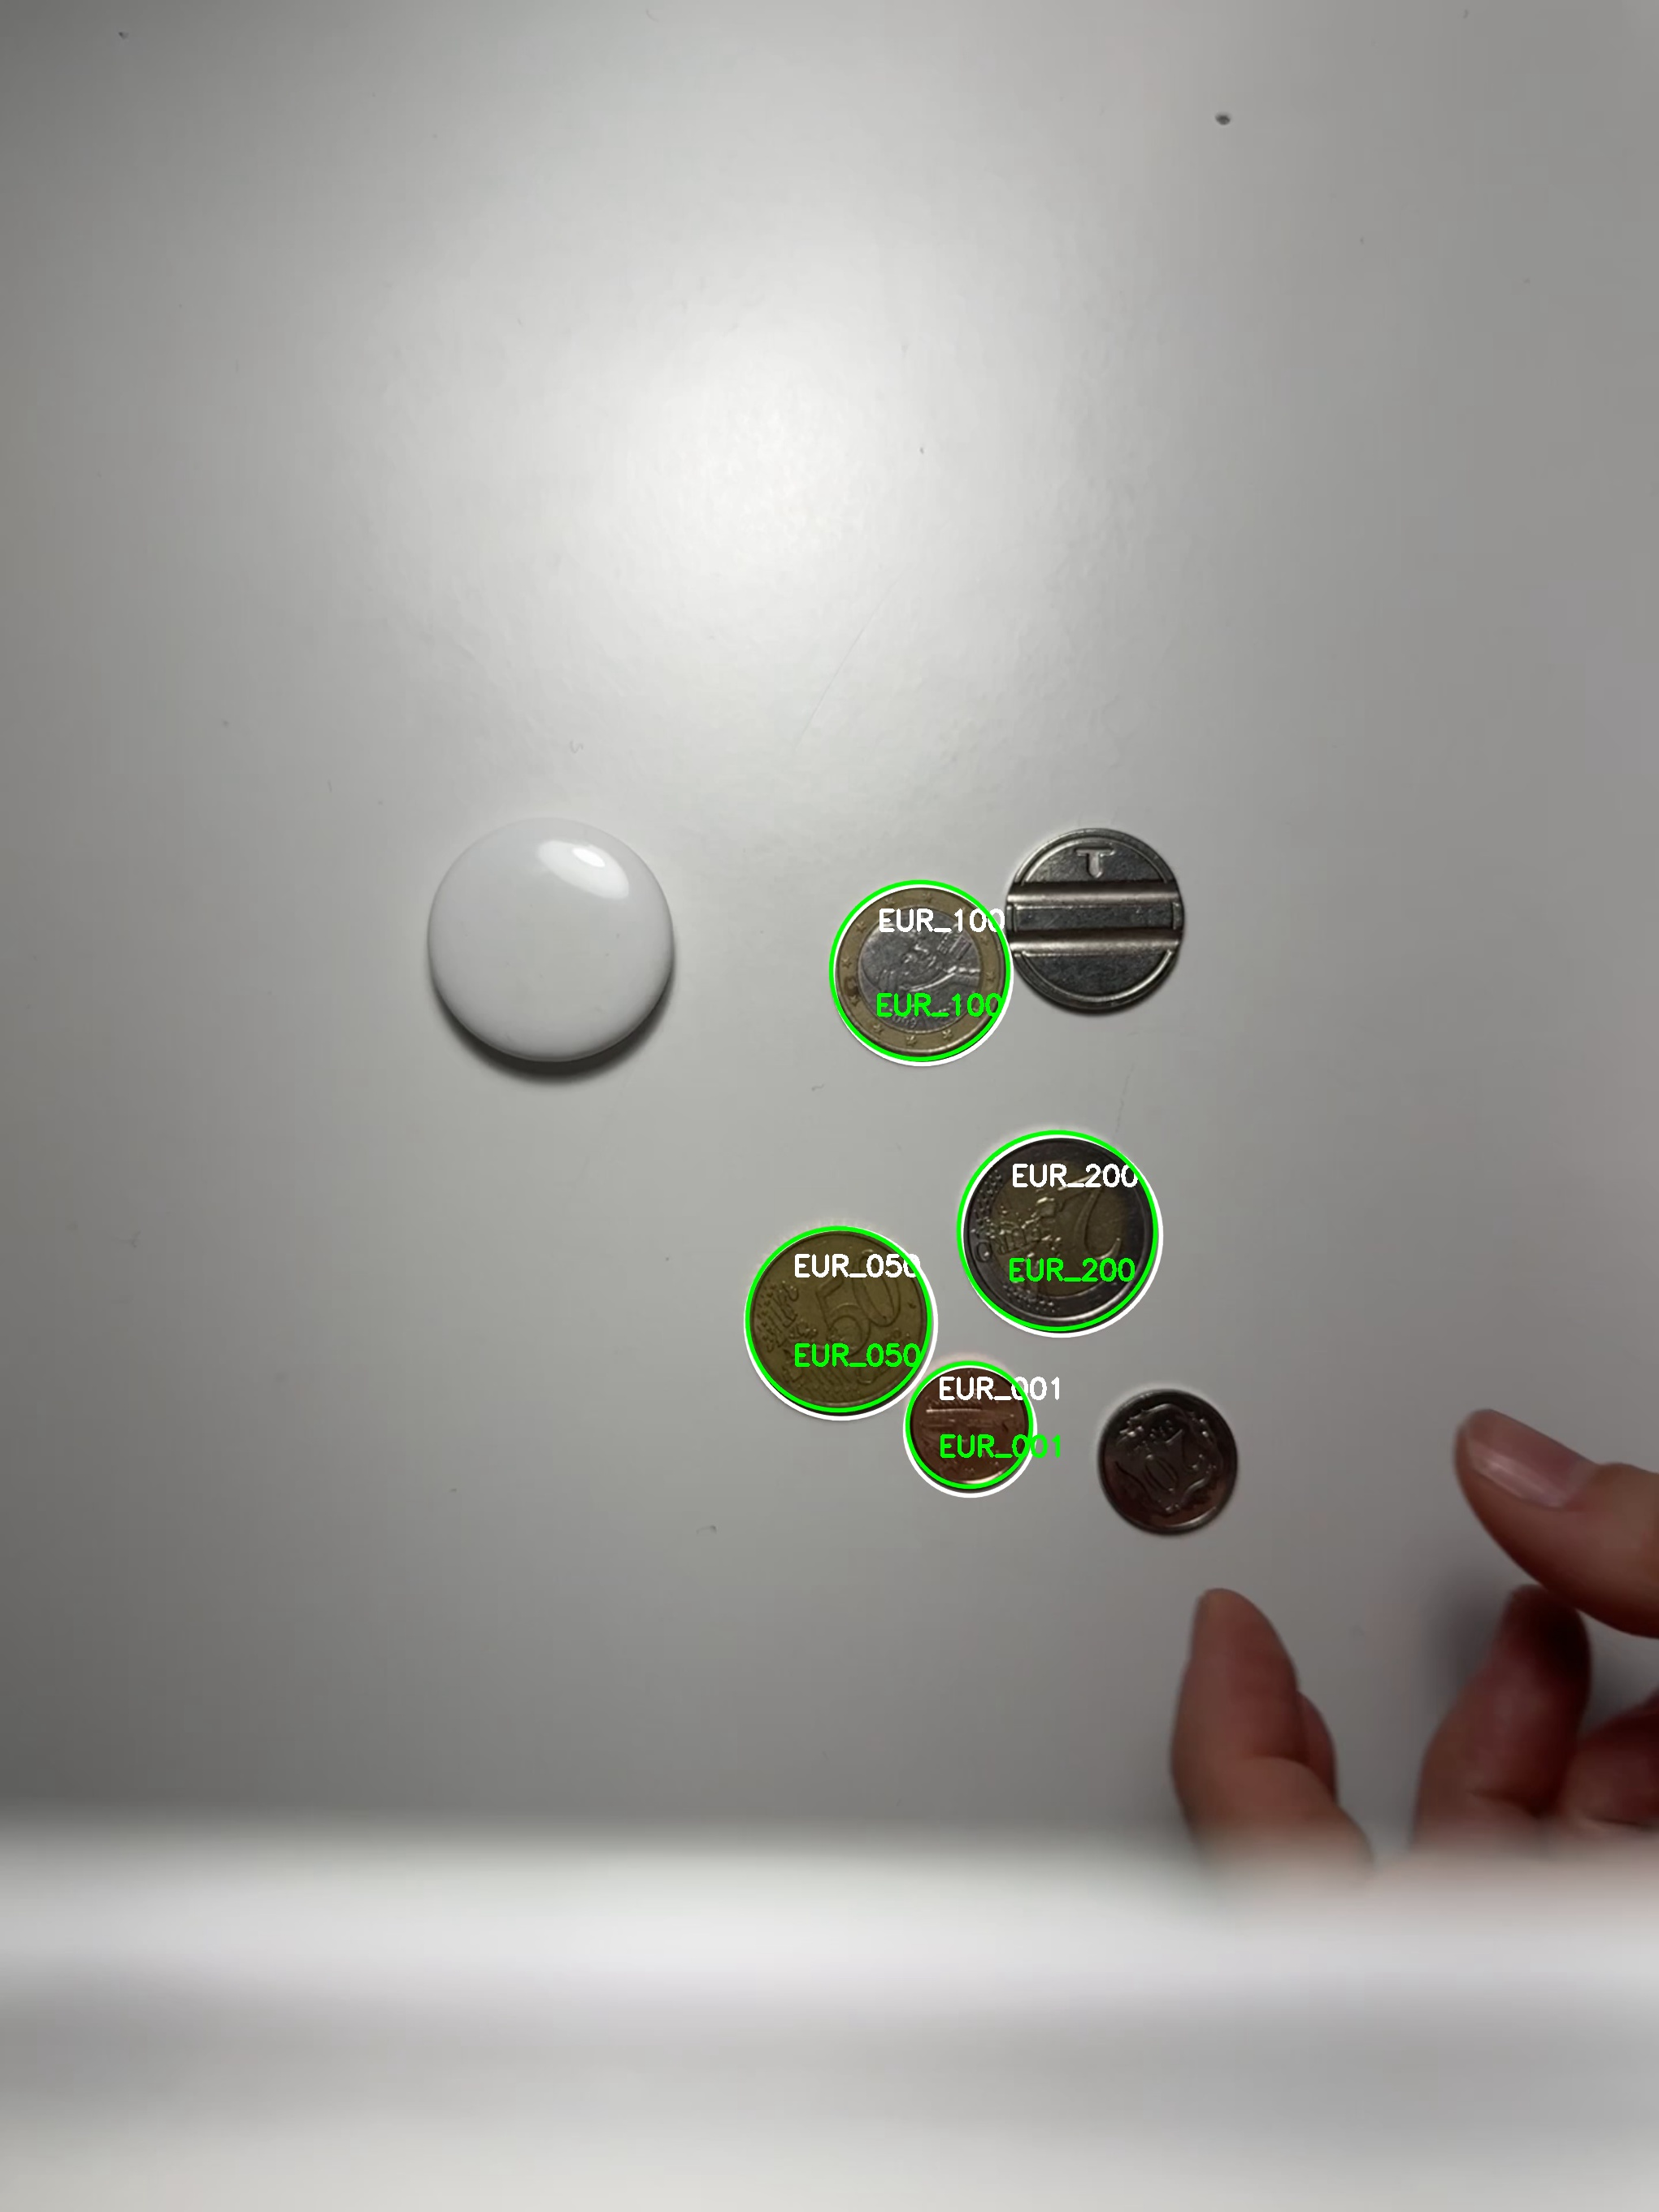
\includegraphics[width=0.45\textwidth]{Immagini/video2_frame_1.jpg}
    }
\end{figure}
\begin{figure}[H]
    \addtocounter{figure}{1} % per non saltare il numero
    \ContinuedFloat
    \centering
    \subfloat[\label{Results:fig:video2_frame2}]{
        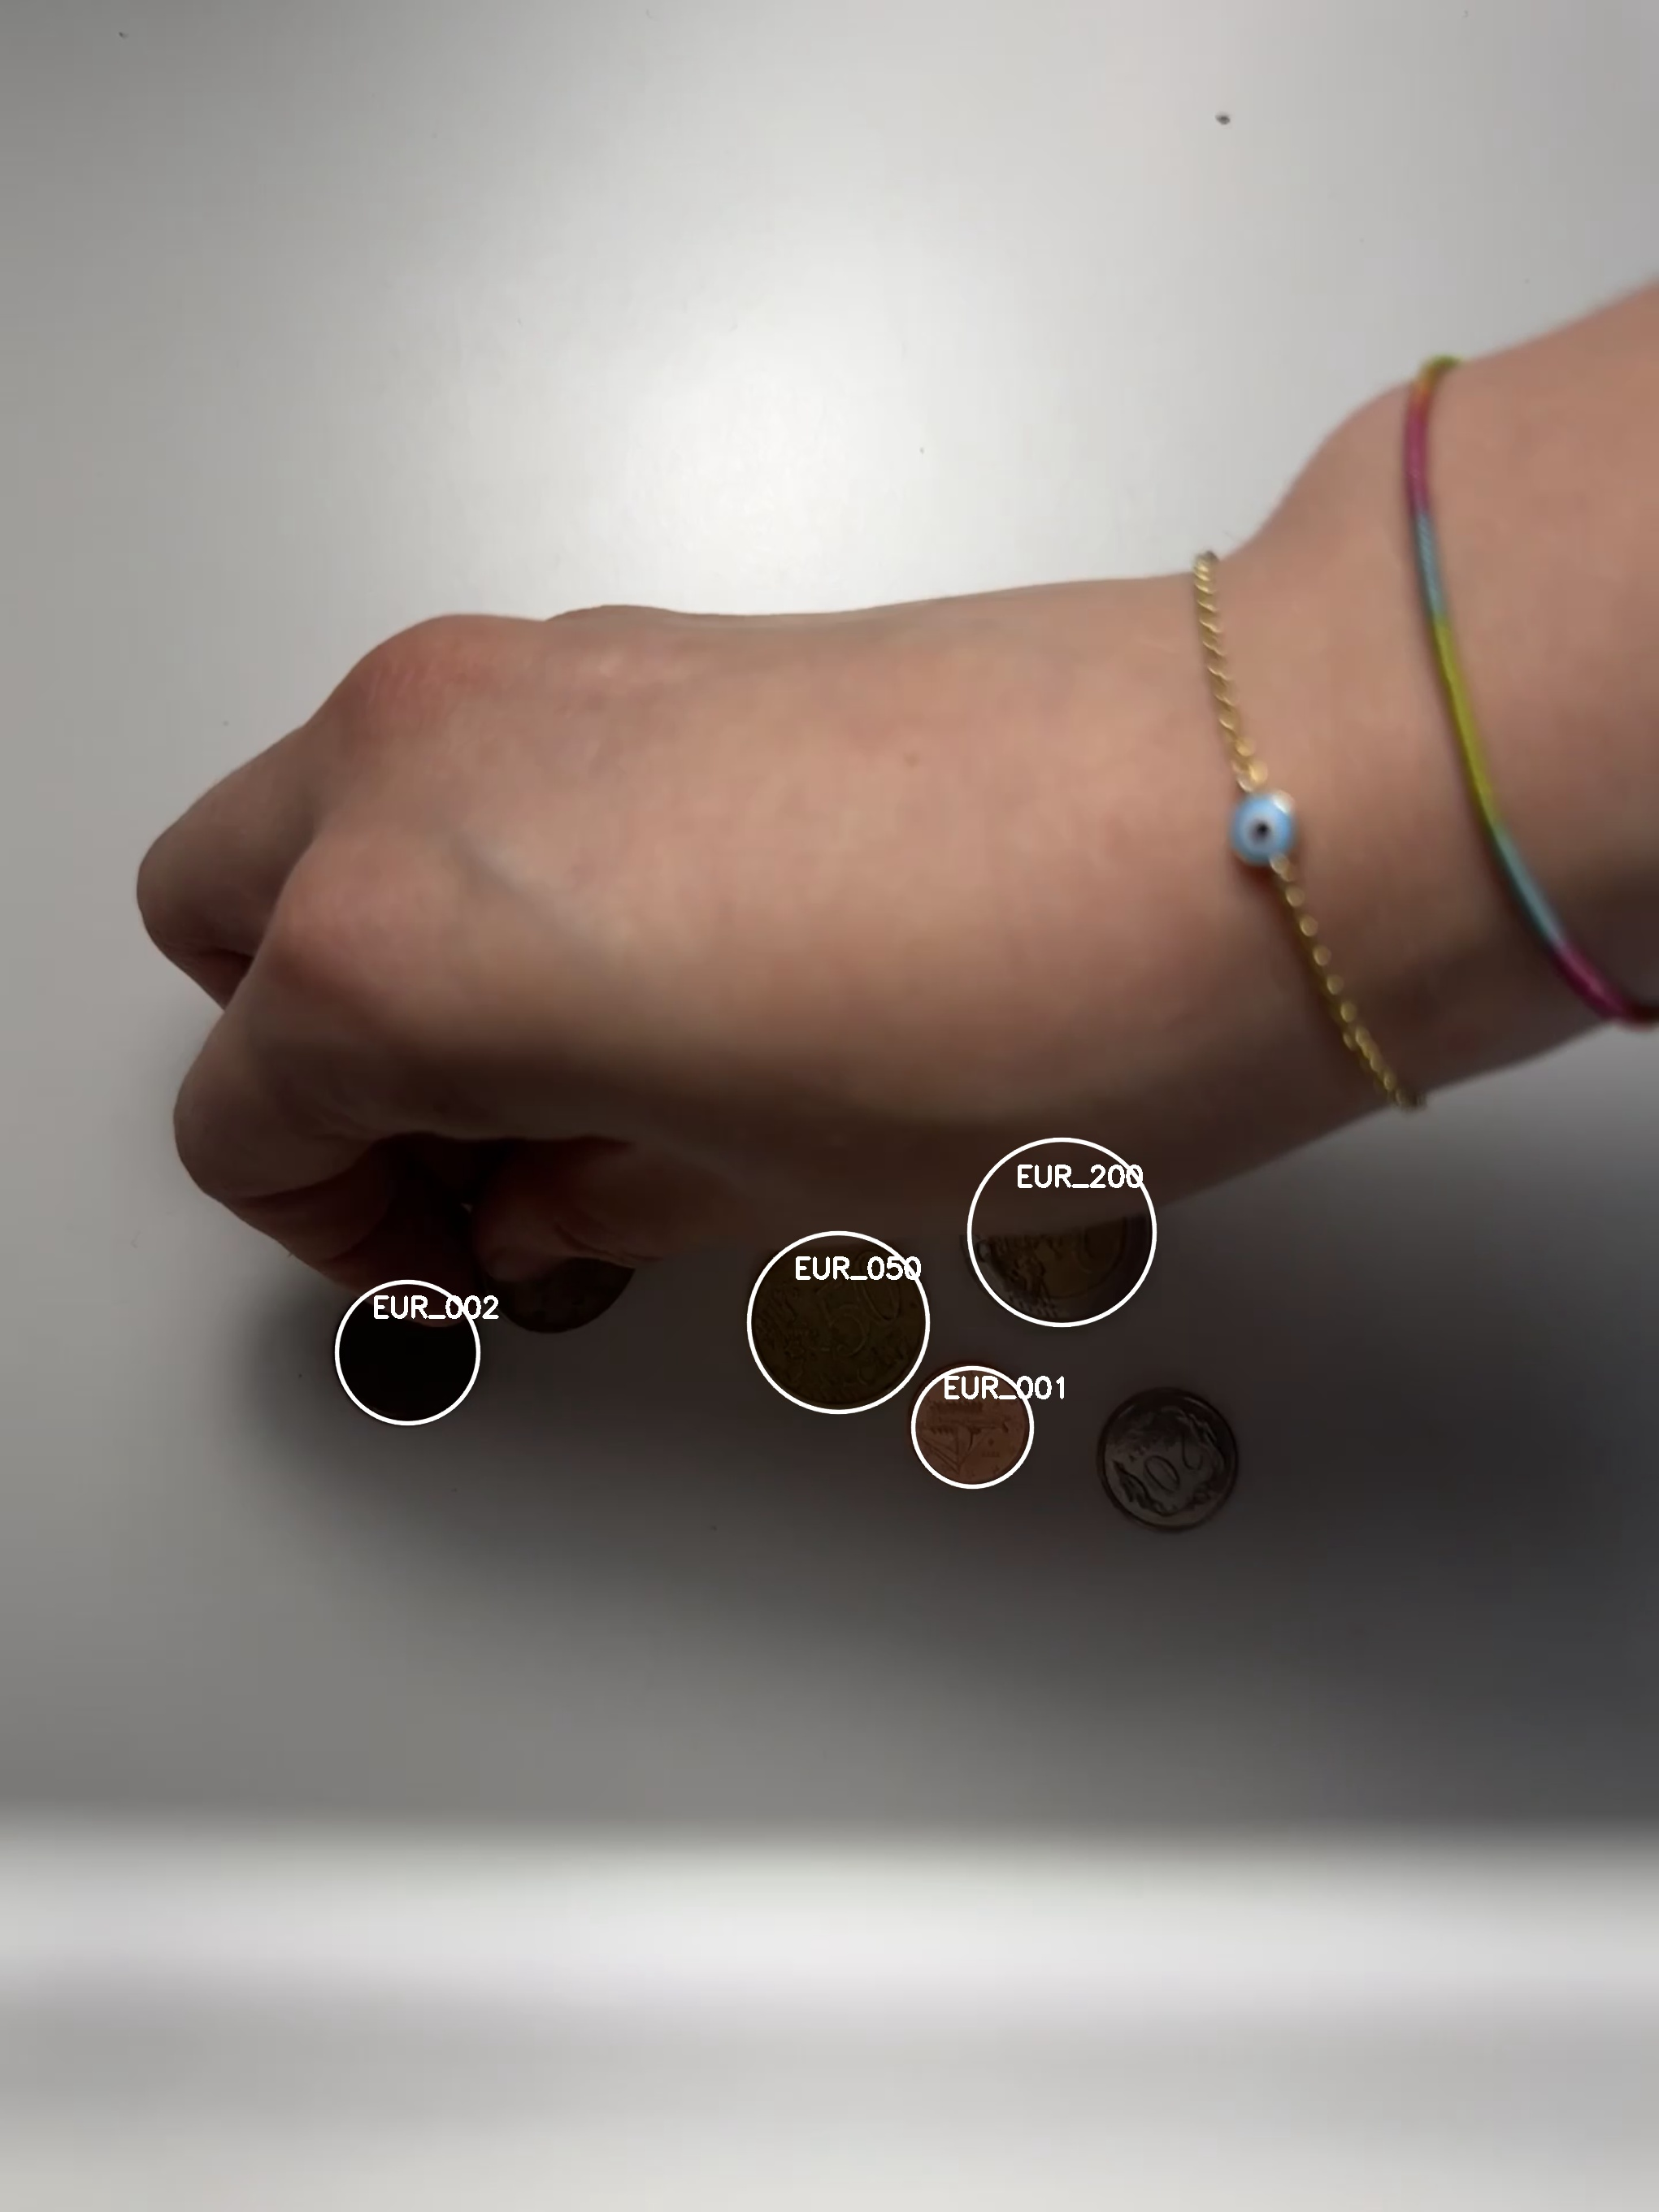
\includegraphics[width=0.45\textwidth]{Immagini/video2_frame_2.jpg}
    }\hfill
    \subfloat[\label{Results:fig:video2_frame3}]{
        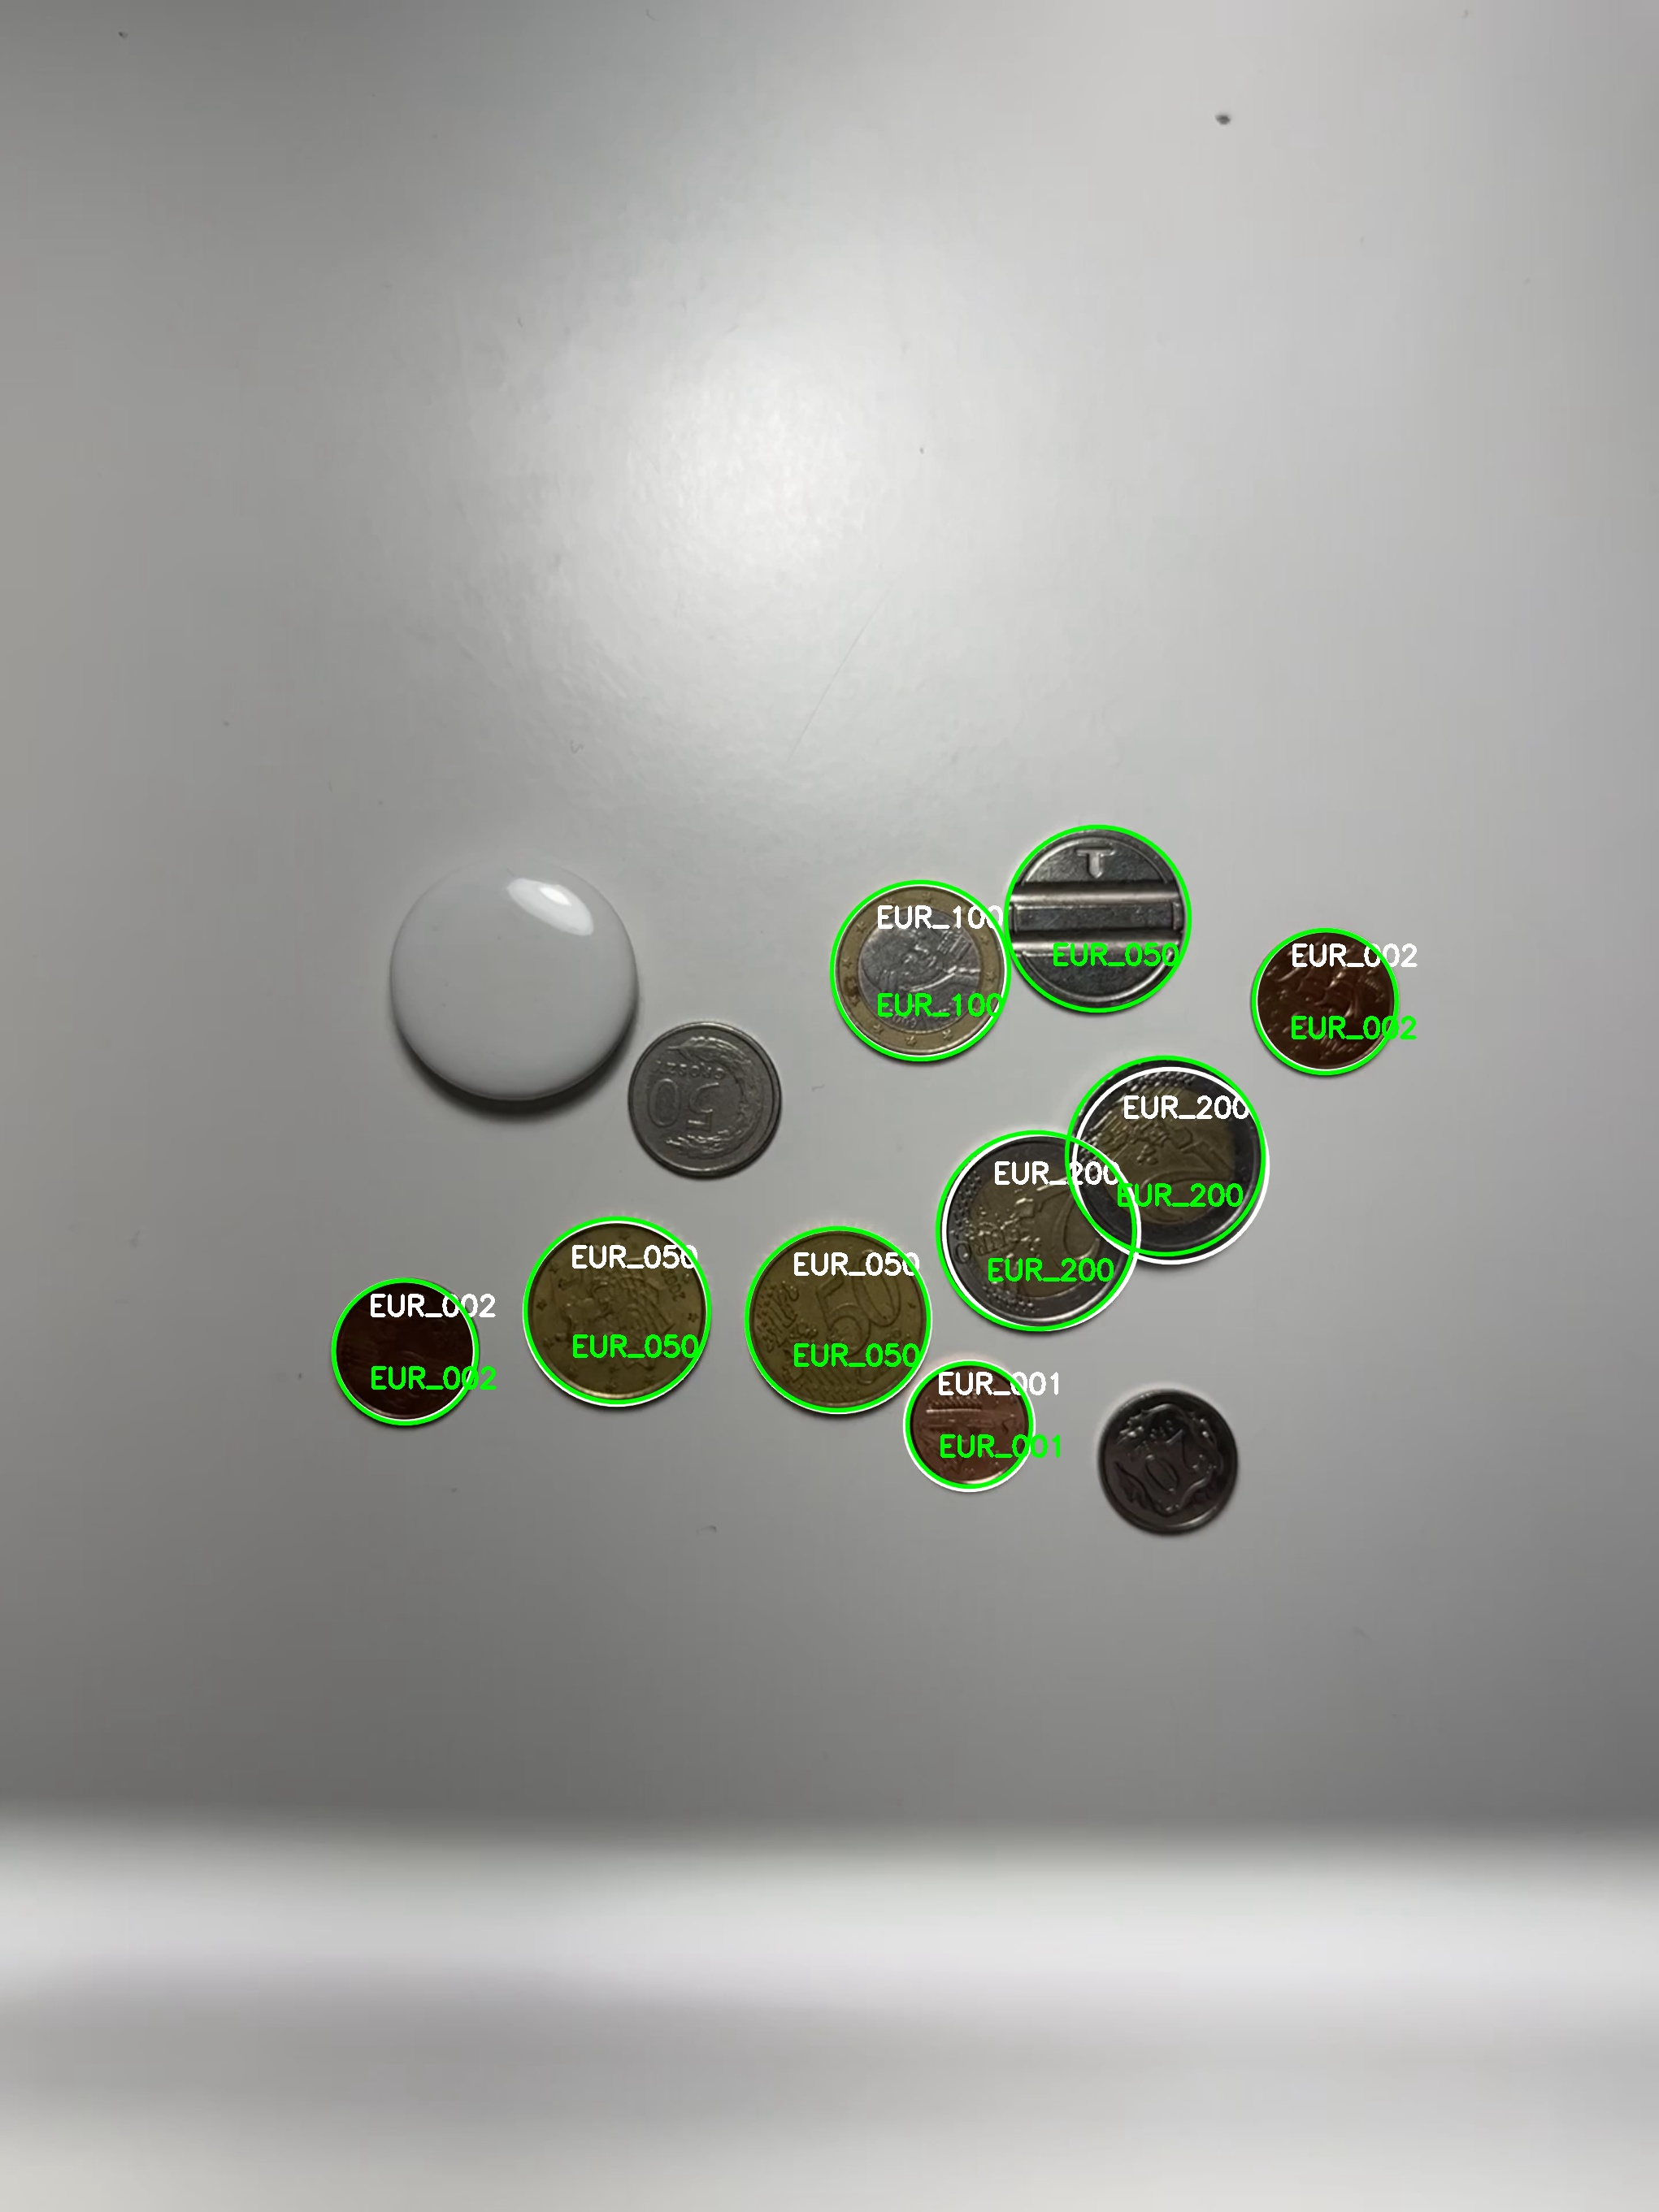
\includegraphics[width=0.45\textwidth]{Immagini/video2_frame_3.jpg}
    }
\end{figure}
\begin{figure}[H]
    \ContinuedFloat
    \centering
    \subfloat[\label{Results:fig:video2_frame4}]{
        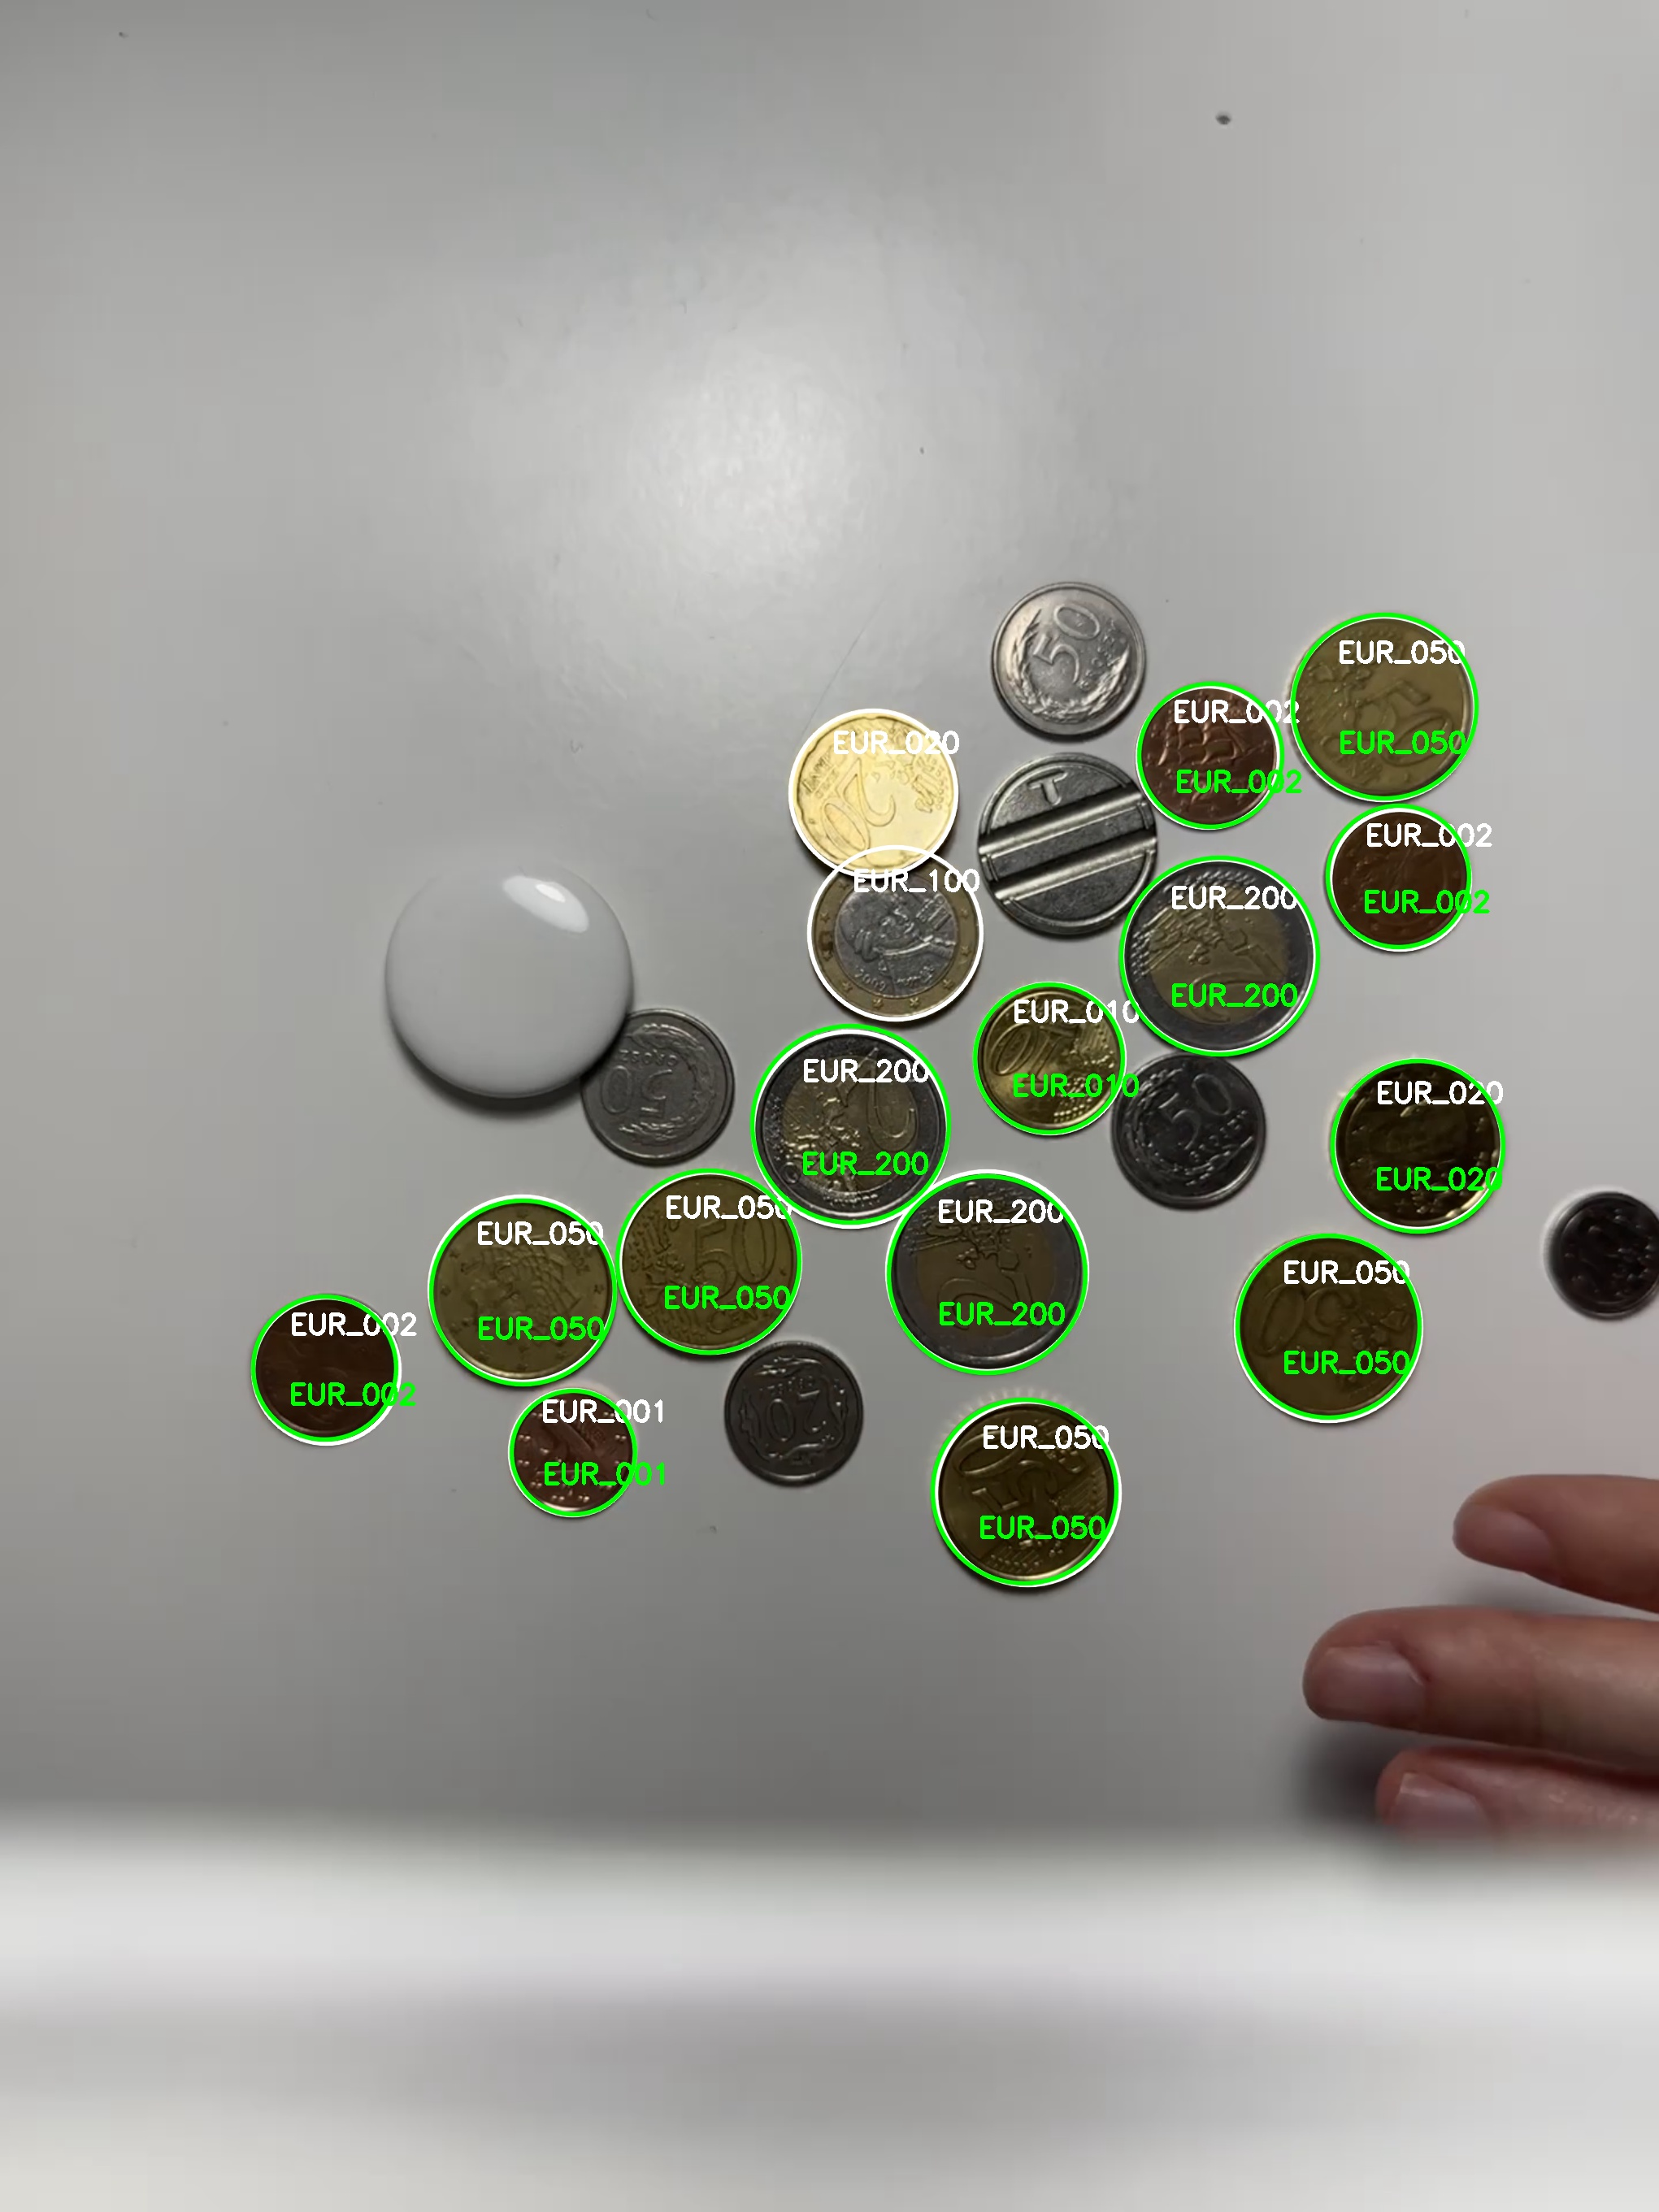
\includegraphics[width=0.45\textwidth]{Immagini/video2_frame_4.jpg}
    }
    \caption{Results of the detection algorithm on selected frames from video 2.
    The ground truth circles are drawn in white, while the detected ones are drawn in green.}
    \label{Results:fig:video2}
\end{figure}